%%%%%%%%%%%%%%%%%%%%%%%%%%%%%%%%%%%%%%START PREAMBLE THAT IS THE SAME FOR ALL EXAMPLES
\documentclass{article}

\usepackage{Sweave}
\usepackage{graphicx}
\usepackage{tabularx}
\usepackage{hyperref}
\usepackage{natbib}
\usepackage{pdflscape}
\usepackage{array}
\usepackage{gensymb}
\usepackage{amsmath}
\usepackage{changepage}
%\usepackage{longtable}
\usepackage{xr}

%\usepackage[backend=bibtex]{biblatex}
%Strongly recommended
%put your figures in one place
%\SweaveOpts{prefix.string=figures/, eps=FALSE} 
%you'll want these for pretty captioning
\usepackage[small]{caption}

\setkeys{Gin}{width=0.8\textwidth}  %make the figs 50 perc textwidth
\setlength{\captionmargin}{30pt}
\setlength{\abovecaptionskip}{10pt}
\setlength{\belowcaptionskip}{10pt}
% manual for caption  http://www.dd.chalmers.se/latex/Docs/PDF/caption.pdf
\topmargin -1.5cm        
\oddsidemargin -0.04cm   
\evensidemargin -0.04cm  % same as oddsidemargin but for left-hand pages
\textwidth 16.59cm
\textheight 21.94cm 

\pagestyle{empty}       
% Uncomment if don't want page numbers
\parskip 7.2pt           % sets spacing between paragraphs
%\renewcommand{\baselinestretch}{1.5} 	% Uncomment for 1.5 spacing between lines
\parindent 0pt% sets leading space for paragraphs
\usepackage{setspace}
%\doublespacing

%%%%%%%%%%%%%%%%%%%%%%%%%%%%%%%%%%%%%%END PREAMBLE

%Start of the document
\begin{document}

%\SweaveOpts{concordance=TRUE}

\bibliographystyle{../refs/bibstyles/amnat.bst}

\title{Supplemental materials for `Shifting phenology of an endangered apex predator tracks changes in its favored prey'}
\date{ }
\maketitle
\author{}
%%%%%%%%%%%%%%%%%%%%%%%%%%%%%%%%%%%%%%%%%%%%%%%%%%%
\renewcommand{\thetable}{S\arabic{table}}
\renewcommand{\thefigure}{S\arabic{figure}}
\section*{Additional details on our use of the Orca Master dataset}

As a presence-only database, trends in the Orca Master dataset should be interpreted with care, since they could be due to shifts in effort (i.e., the number of total observations) as well as (or instead of) trends in SRKW presence (see Effects of changes in effort on estimated phenological change in the Supplemental Materials). For this reason, and because we know there has been a dramatic increase in reported whale sightings (Olson et al., 2018), we report all trends across two different durations: the full dataset (from 1978-2017) and recent years (2001-2017). We use 2001 as a cut-off, to avoid the sharp increase in sightings that occurred from 2000 to 2001 (Fig. S3-4), likely influenced by the onset of internet-based sightings platforms that began that year \citep{hauser2007,olson2018}.

For our analyses, observation of any individual or group of whales within a pod counted as presence of that pod, with the exception of ``L87,'' an individual that spent little time with his natal L pod following the death of his mother, and was instead seen more frequently with J- and K-pods. Observations of this individual alone were therefore not counted as presence of L pod in our analyses.
 
\section*{Models}
\emph{Southern resident killer whale presence and their prey at Lime Kiln Point State}
\begin{enumerate}
\item \underline{Southern resident killer whale presence model}
\par We fit a separate hierarchical model to each pod (J, K, L), as well as a hierarchical model to all SRKWs pooled together. We estimated the presence, or occurrence probability (with presence when Pr(\emph{$\psi$}=1)), as a smooth function of day of year, \emph{s(day)}. Specifically, we assumed $\psi$ to be a Bernoulli random variable dependent on day of year (as a smooth function, using thin plate regression spline basis), with a year-specific shape as well as a year-specific intercept (i.e., a random effect of year):


\begin{align*}
Pr(\psi_i = 1) &= logit^{-1} (\alpha_{year[i]} + s(day)_{year[i]})
\end{align*}

\begin{align*}
\alpha_{year} & \sim N(\mu_{\alpha}, \sigma^{2}_{\alpha}) \\
\end{align*}


\item \underline{Fraser River Chinook salmon abundance index model}

We modeled an index of Fraser River Chinook salmon abundance (\emph{y}, the log of the daily catch per unit effort [CPUE] to which we added 0.001 prior to logging to avoid values of zero) as a smooth function of day of year (using thin plate regression spline basis), with a year-specific shape as well as a year-specific intercept (i.e., random effect of year):


\begin{align*}
y_i &= \alpha_{year[i]} + s(day)_{year[i]}
\end{align*}

\begin{align*}
\alpha_{year} & \sim N(\mu_{\alpha}, \sigma^{2}_{\alpha}) \\
\end{align*}

\end{enumerate}

The above models for killer whales ad Chinook were fitted via thin plate regression spline basis using the programming language \texttt{Stan} \citep{Carpenter:2016aa} (\texttt{www.mc-stan.org}), accessed via the \texttt{brms}\citep{brms2018} package in R \citep{Rcore2021}, version 4.0.4. For each model fit, we ran four chains simultaneously, each with 4 000 sampling iterations (1 000 of which were used for warm-up). Code for the above models is in Appendix 1. We assessed model performance through $R_{hat}$ (all were close to 1) and high neff, as well as visual consideration of chain convergence and posteriors \citep{BDA}.
\par \emph{Southern resident killer whales and salmon in the Central Salish Sea and Puget Sound Proper}
\begin{enumerate}
\item \underline {Southern resident killer whale occupancy models}
\par We quantified pod-specific phenology for J, K, and L pods using occupancy models, which can estimate jointly species presence and detection probability (p, the probability of detecting at least one individual present at a site) by distinguishing true presence or absence, \emph{z} (a latent, unobservable state), from observed presence. Occupancy models are composed of a state sub-model, which is the model for the ecological process of true presence or absence, and an observation sub-model, which in this case links the observations (i.e., the number of sightings of the pod per day per site) to the state model. We modeled occupancy probability ($\psi_{year,day}$) as a semi-parametric, smooth function of day of year (\emph{`day'}), using flexible thin-plate spline regression modeling, and year as a level \citep{strebel2014}. Thus, the sub-models are:
\begin{itemize}

\item \textbf{State model}, in which we assumed $Z_{year,day}$ to be a Bernoulli random variable for which 0 signifies absence and 1 is presence:
 \begin{align*}
Z_{year,day} \sim Bernoulli (\psi_{year,day})
\end{align*}
  \item \textbf{Observation model}, in which the number of successful sightings ($Y$) in a particular fishing area on a particular day in a particular year, was modeled as a binomial random variable composed of the total number of sightings made in the area, year, and day ($T_{year,day,area}$), and the product of the state of occurrence ($Z_{year,day}$) and detection probability ($P$). We modeled detection probability as a year- and area-specific probability between 0 and 1 ($P_{area,year}$):
\begin{align*}
Y(area,year,day) \sim Binomial (T_{year, day,area},Z_{year,day}*P_{area,year})
\end{align*}
                                                                             \end{itemize}                                                       

 
\par We fit separate occupancy models for each region (i.e., Central Salish Sea and Puget Sound proper) and season (spring/summer vs. fall/winter, since seasonal use varies by region) for each pod, and extracted estimates of annual arrival, departure, and peak occupancy dates with each model. We defined the arrival date as the earliest day within the season when occupancy probability exceeded 0.5; departure date was the latest day within the season when detection probability exceeded 0.5. Using a threshold probability between 0.2 and 0.5 did not qualitatively alter observed trends.) Pod-specific occupancy models were fit using \texttt{JAGS}, a program for analysis of Bayesian hierarchical models with Markov Chain Monte Carlo simulation (Plummer, 2019), accessed via the \texttt{R2jags} package \citep{su2021} in R \citep{Rcore2021}, version 4.0.0. We ran four chains simultaneously, each with 12 000 sampling iterations (4 000 of which were used for burn-in). We assessed model performance through $R_{hat}$, which were close to 1, and high neff, as well as visual consideration of chain convergence and posteriors \citep{BDA}. Model code can be found in Appendix 2.
\item \underline {Salmon abundance index models}
\par To estimate the phenology of likely prey in the Central Salish Sea, we fit the hierarchical thin-plate regression spline models described above to the Albion Test Fishery data, from May through October (the full seasonal extent of the dataset), and from 1994 through 2017. To estimate the phenology of likely prey in Puget Sound, we fit the hierarchical thin-plate regression spline models separately to each of 13 Puget Sound runs (including three species across hatchery and wild salmon in 7 streams, Table \ref{tab:salmon}) and used daily abundance index estimates to identify the day of year of first, peak, and last migration for each group in each year. We then used hierarchical linear models to identify trends over time in phenology of salmon adult migration timing across Puget Sound proper.  We fit  separate multi-level linear models to each phenophase to estimate trends across years in the timing of adult salmon migration. The response variable, \emph{day} is the day of year of the event (i.e., first, peak, or last date of migration in a given year) and the explanatory variable was year; we included group as a random effect to account for non-independence in timing at the group-level, as follows:

\begin{align*}
day_i &= \alpha_{group[i]} + \beta_{year}
\end{align*}

\begin{align*}
\alpha_{group} & \sim N(\mu_{\alpha}, \sigma^{2}_{\alpha}) \\
\end{align*}

\end{enumerate}
See Appendices for model code.

\section* {Comparing observed and modeled estimates of `whale days' at Lime Kiln Point State Park, Washington, USA}
\par We calculated annual total whale days quantified from the data directly (i.e., a whale-day was counted as a day on which Southern Resident Killer Whales (SRKWs) were observed) and quantified from model-estimated probabilities of whale presence (i.e., each days probability of whale presence was summed across the year). Model-estimated presence probabilities were obtained from occupancy models, which estimated daily and annual probabilities of presence of SRKWs at Lime Kiln Point State Park. The two calculations were similar, and both reveal declines in SRKW presence in recent years, across all three pods (Fig. \ref{fig:mlimewdays}). This consistently collected dataset also suggests that SRKWs have shifted the timing of their activity in the area (Fig. 3 in the main text).

\section* {Effects of changes in effort on estimated phenological change}
With increasing public awareness of SRKWs near urban areas (e.g. the Salish Sea), the number of public reports of whales and people contributing to sightings networks such as the Orca Master Database have increased since its inception (Fig.\ref{fig:sights}). This shift in effort complicates interpretations of trends in the number of whale days over time (Fig. \ref{fig:wdays}) because an increase in the number of whale on which SRKWs were observed could be due to increased observer effort in a region, rather than due to increased whale activity in the region. To better understand how increased effort across the time-series (i.e., increased numbers of sightings over time) may affect estimates of trends in phenology, we simulated data sets of whale presence during two seasons equivalent to those in our data set (spring/summer, which was 1 May through 31 Sept, or 153 days, and fall/winter, which was 1 October through 1 Feb, or 123 days). We used whale presence probabilities that matched the mean observed probabilities for the Central Salish Sea and Puget Sound regions, separately, from 1978-2017 (Table S1). We kept them constant over 40 simulated years, respectively. We then created an observation data set, in which effort (the number of observations) varied. During the low effort time period (years 1-20), the number of observations had a mean of 15 per year for Puget Sound and 104 per year in the Central Salish Sea (matching the means for these regions from 1978-1997 in the Orca Master database). During the high effort time period (years 21-40 in our simulated data set), the number of annual observations had a mean of 39 for Puget Sound and 133 for the Central Salish Sea (matching those in the Orca Master database from 1998-2017). We then calculated first- and last- observations dates for each simulated year. We ran these simulations 100 times and calculated the difference between the low effort and high effort time periods. We compared these to the mean differences in first- and last-observation dates across time periods in the Orca Master database, for each region, to understand whether observed changes may be due to changes in effort over time, rather than changes in killer whale activity. We conducted the same analysis across the recent time frame (2001-2017), as well, using region-specific estimates of presence probabilities and observer effort obtained from this time-period.

\par Our simulations indicate that, if SRKW activity did not change and only effort changed across the two time-periods, the first observation would be expected to shift earlier from 1978-2017, especially in Puget Sound (Fig.\ref{fig:simeffort}A), perhaps because the number of sightings was very low early in the time-series. Thus, the large increase in effort across this time period may affected trends in phenological shifts.  However, the expected change due to increased effort opposes the patterns we observed in for the Central Salish Sea (i.e., we would expect earlier arrival and later departure). Further, focusing on 2001-2017 only, effects of changes in effort are likely to be minimal (Fig.\ref{fig:simeffort}B). Due to the presence only nature of the Orca Master Database, it is difficult to fully separate an absence of whales from an absence of observers. We therefore focus our interpretation on the recent time-period (2001-2017).

\bibliography{..//refs/noaalib.bib}

%\par Coincident with these phenological trends, the number of whale days has also changed across the time-series (Fig. SX). Since 2001, the number of whale days has decreased in the Central Salish Sea, across all pods, whereas in Puget Sound proper the number of whale days did not show a consistent trend (Fig. SX). From 1978 to 2017, the number of whale days increased in both regions (and for all pods). 

\pagebreak

\section* {Supplemental Tables}
% latex table generated in R 4.0.4 by xtable 1.8-4 package
% Thu Oct 21 13:37:50 2021
\begin{table}[ht]
\centering
\caption{\textbf{Data types and sources}} 
\label{tab:salmon}
\begingroup\footnotesize
\begin{tabular}{|p{0.1\textwidth}|p{0.1\textwidth}|p{0.2\textwidth}|p{0.16\textwidth}|p{0.2\textwidth}|p{0.16\textwidth}|}
  \hline
Region & Species & Data Source & Data Type & Spatial Scale & Temporal Scale \\ 
  \hline
Central Salish Sea & SRKW & Lime Kiln Point State Park & Standardized effort & Local (single point) & 1994-2017, daily May-Sept \\ 
   & SRKW & Orca Master (The Whale Museum, 2018) & Presence-only, crowd-sourced & Regional (multiple points) & 1978-2017, opportunistic observations \\ 
   & Chinook salmon & Albion test fisher & Standardized effort & Local (transect) & 1992-2017, daily April-Oct \\ 
   \hline
Puget Sound Proper & SRKW & Orca Master (The Whale Museum, 2018) & Presence-only, crowd-sourced & Regional (multiple points) & 1978-2017, opportunistic observations \\ 
   & Chinook,coho, chum salmon & WDFW count data from 7 streams & Standardized effort & Local (13 points) & Variable (see Table S2) \\ 
   \hline
\end{tabular}
\endgroup
\end{table}
% latex table generated in R 4.0.4 by xtable 1.8-4 package
% Thu Oct 21 13:37:50 2021
\begin{table}[ht]
\centering
\caption{\textbf{Salmon runs in Central Salish Sea and Puget Sound Proper} included in our analyses.} 
\label{tab:salmon}
\begingroup\footnotesize
\begin{tabular}{|p{0.16\textwidth}|p{0.3\textwidth}|p{0.06\textwidth}|p{0.1\textwidth}|p{0.06\textwidth}|p{0.08\textwidth}|}
  \hline
Region & Location & Species & Origin & Latitude & Longitude \\ 
  \hline
Central Salish Sea & ALBION TEST FISHERY & Chinook & wild/hatchery & 49.2104 & -122.6228 \\ 
   \hline
Puget Sound Proper & CEDAR RIVER HATCHERY & Chinook & wild & 47.3761 & -121.9625 \\ 
   & CEDAR RIVER HATCHERY & coho & wild & 47.3761 & -121.9625 \\ 
   & GARRISON HATCHERY & chum & wild & 47.1915 & -122.5741 \\ 
   & GEORGE ADAMS HATCHERY & chum & hatchery & 47.3013 & -123.1818 \\ 
   & GEORGE ADAMS HATCHERY & Chinook & hatchery & 47.3013 & -123.1818 \\ 
   & HOODSPORT HATCHERY & chum & hatchery & 47.407 & -123.1399 \\ 
   & HOODSPORT HATCHERY & Chinook & hatchery & 47.407 & -123.1399 \\ 
   & MCKERNAN HATCHERY & chum & hatchery & 47.3066 & -123.203 \\ 
   & MINTER CR HATCHERY & chum & hatchery & 47.3726 & -122.7026 \\ 
   & MINTER CR HATCHERY & Chinook & hatchery & 47.3726 & -122.7026 \\ 
   & MINTER CR HATCHERY & coho & wild & 47.3726 & -122.7026 \\ 
   & MINTER CR HATCHERY & coho & hatchery & 47.3726 & -122.7026 \\ 
   & SOOS CREEK HATCHERY & chum & wild & 47.3093 & -122.1688 \\ 
   \hline
\end{tabular}
\endgroup
\end{table}\begin{adjustwidth}{-4cm}{-2cm}
% latex table generated in R 4.0.4 by xtable 1.8-4 package
% Thu Oct 21 13:37:50 2021
\begin{table}[ht]
\centering
\caption{\textbf{Salmon phenology has shifted} later in part of the Central Salish Sea (based on spring/summer Chinook in the Albion Test Fishery data, from 1995-2017) and earlier in Puget Sound Proper (based on 13 runs across coho, chum, and Chinook adult in Table S1, from 1997-2017). Estimated linear trends are shown for peak, first, and last likely occurrance dates for salmon.  `Peak' is the day of year with the maximum estimated abundance index.   To  estimate  the  start  of  the  season,  we  identified  the earliest day of year with an estimated abundance index >0.001 catch per unit effort (CPUE) for Albion test fishery data in the central Salish Sea, and fish counts greater than  0 for Puget Sound stream counts.  To estimate the end of the season, we identified the latest day of year CPUE or count greater than these values.  50 percent, 75 percent, and 95 percent uncertainty intervals are shown.} 
\label{tab:salmtren}
\begingroup\tiny
\begin{tabular}{|p{0.16\textwidth}|p{0.05\textwidth}p{0.05\textwidth}p{0.05\textwidth}p{0.05\textwidth}p{0.05\textwidth}p{0.05\textwidth}p{0.05\textwidth}p{0.05\textwidth}p{0.05\textwidth}|}
  \hline
region & season & phase & mean & 25\% & 75\% & 12.5\% & 87.5\% & 2.5\% & 97.5\% \\ 
  \hline
Central Salish Sea & sum & peak & 0.815 & 0.709 & 0.922 & 0.631 & 0.999 & 0.492 & 1.139 \\ 
   & sum & first & 3.331 & 2.861 & 3.802 & 2.52 & 4.143 & 1.903 & 4.76 \\ 
   & sum & last & -0.071 & -0.174 & 0.032 & -0.249 & 0.107 & -0.385 & 0.243 \\ 
   \hline
Puget Sound Proper & fall & peak & -0.318 & -0.416 & -0.22 & -0.486 & -0.15 & -0.605 & -0.031 \\ 
   & fall & first & -0.719 & -0.859 & -0.579 & -0.958 & -0.48 & -1.128 & -0.311 \\ 
   & fall & last & -0.659 & -0.755 & -0.562 & -0.823 & -0.494 & -0.94 & -0.377 \\ 
   \hline
\end{tabular}
\endgroup
\end{table}
\vspace*{\floatsep}

% latex table generated in R 4.0.4 by xtable 1.8-4 package
% Thu Oct 21 13:37:50 2021
\begin{table}[ht]
\begin{flushleft}
\caption{\textbf{Estimated linear trends in peak, first, and last likely occurance dates for southern resident killer whiles} in Puget Sound proper (`ps') during the fall/winter (`fall', from July through December) and the central Salish Sea (`css') during the spring/summer (`sum', from April through October), from occupancy model estimates of presence probabilites. `Peak' is the day of year with the maximum probability of presence (or the mean across day of year, if there are multiple days with the same peak probability of presence). To estimate the start of the season, we identified the earliest day of year with an estimated presence probility greater than 0.5. To estimate the end of the season, we identified the latest day of year with an estimated presence probility greater than 0.5. 50 percent, 75 percent, and 95 percent uncertainty intervals are shown.} 
\label{tab:modsum}
\begingroup\tiny
\begin{tabular}{|p{0.018\textwidth}|p{0.035\textwidth}|p{0.035\textwidth}|p{0.035\textwidth}|p{0.035\textwidth}p{0.035\textwidth}p{0.035\textwidth}p{0.035\textwidth}p{0.035\textwidth}p{0.035\textwidth}p{0.035\textwidth}|p{0.035\textwidth}p{0.035\textwidth}p{0.035\textwidth}p{0.035\textwidth}p{0.035\textwidth}p{0.035\textwidth}p{0.035\textwidth}|}
  \hline & & & & \multicolumn{7}{c |}{1978-2017 trend} &\multicolumn{7}{c |}{2001-2017 trend}\\
 pod & region & season & phase & mean & 25\% & 75\% & 12.5\% & 87.5\% & 2.5\% & 97.5\% & mean & 25\% & 75\% & 12.5\% & 87.5\% & 2.5\% & 97.5\% \\ 
  \hline
J & css & sum & peak & 1.01 & 0.60 & 1.43 & 0.71 & 1.61 & -0.19 & 2.18 & 6.49 & 3.96 & 9.48 & -1.41 & 2.38 & -4.05 & 14.90 \\ 
  J & css & sum & first & -0.76 & -0.90 & -0.61 & -0.25 & 1.28 & -1.21 & -0.32 & 1.10 & 0.94 & 1.21 & 0.61 & 4.24 & 0.70 & 1.79 \\ 
  J & css & sum & last & 1.12 & 0.96 & 1.28 & 0.20 & 1.73 & 0.70 & 1.63 & 0.39 & 0.21 & 0.60 & -2.80 & 0.22 & -0.13 & 0.90 \\ 
  J & ps & fall & peak & 1.17 & 0.91 & 1.47 & 0.26 & 1.71 & 0.33 & 1.93 & 0.45 & -0.67 & 1.55 & 0.95 & 11.28 & -2.81 & 4.09 \\ 
  J & ps & fall & first & 0.53 & 0.06 & 1.00 & -1.01 & -0.51 & -0.81 & 1.82 & 2.44 & 1.37 & 3.45 & 0.86 & 1.31 & -0.59 & 5.51 \\ 
  J & ps & fall & last & 0.95 & 0.49 & 1.40 & 0.86 & 1.40 & -0.32 & 2.27 & -1.23 & -2.22 & -0.28 & 0.06 & 0.70 & -3.60 & 1.09 \\ 
   \hline
K & css & sum & peak & 0.93 & 0.63 & 1.24 & 1.21 & 2.27 & 0.01 & 1.78 & 1.31 & 0.42 & 2.24 & -0.44 & 3.75 & -1.43 & 3.91 \\ 
  K & css & sum & first & -0.33 & -0.58 & -0.07 & 0.70 & 2.52 & -1.09 & 0.42 & 0.82 & 0.29 & 1.55 & 0.28 & 4.49 & -0.80 & 2.63 \\ 
  K & css & sum & last & 0.65 & 0.42 & 0.85 & 1.80 & 3.69 & 0.09 & 1.30 & -1.00 & -1.57 & -0.57 & 0.39 & 2.33 & -2.05 & 1.06 \\ 
  K & ps & fall & peak & 1.75 & 1.44 & 2.07 & 0.41 & 1.43 & 0.76 & 2.62 & 1.59 & 0.35 & 2.78 & -0.24 & 2.83 & -1.97 & 5.67 \\ 
  K & ps & fall & first & 1.62 & 1.10 & 2.18 & -0.78 & 0.11 & 0.05 & 3.15 & 2.35 & 1.10 & 3.63 & -0.36 & 1.89 & -1.40 & 6.04 \\ 
  K & ps & fall & last & 2.75 & 2.21 & 3.31 & 0.28 & 1.02 & 1.21 & 4.20 & 1.27 & 0.64 & 1.83 & -1.76 & 0.14 & -0.42 & 3.36 \\ 
   \hline
L & css & sum & peak & 0.21 & -0.04 & 0.48 & 0.71 & 1.43 & -0.52 & 0.99 & -1.14 & -2.16 & -0.14 & -1.42 & 0.57 & -4.02 & 1.76 \\ 
  L & css & sum & first & -1.79 & -2.07 & -1.50 & 0.44 & 2.81 & -2.63 & -0.92 & 0.55 & 0.23 & 0.87 & -0.70 & 3.59 & -0.47 & 1.48 \\ 
  L & css & sum & last & 1.09 & 0.85 & 1.30 & -0.30 & 2.28 & 0.47 & 1.81 & -0.20 & -0.40 & 0.02 & -2.93 & -0.75 & -0.88 & 0.38 \\ 
  L & ps & fall & peak & 1.07 & 0.87 & 1.29 & -0.20 & 0.72 & 0.41 & 1.65 & -0.47 & -1.03 & 0.03 & -2.80 & 0.55 & -2.21 & 1.58 \\ 
  L & ps & fall & first & 1.62 & 0.95 & 2.32 & -2.26 & -1.30 & -0.47 & 3.55 & 1.38 & 0.11 & 2.68 & -0.20 & 0.96 & -2.34 & 4.85 \\ 
  L & ps & fall & last & 1.02 & 0.23 & 1.82 & 0.70 & 1.43 & -1.16 & 3.00 & -1.82 & -2.44 & -1.17 & -0.51 & 0.23 & -3.92 & 0.23 \\ 
   \hline
\end{tabular}
\endgroup
\end{flushleft}
\end{table}\end{adjustwidth}





\newpage
\section*{}

\newpage
.
.

\newpage
\section* {Supplemental Figures}

\begin{figure}[!hp]
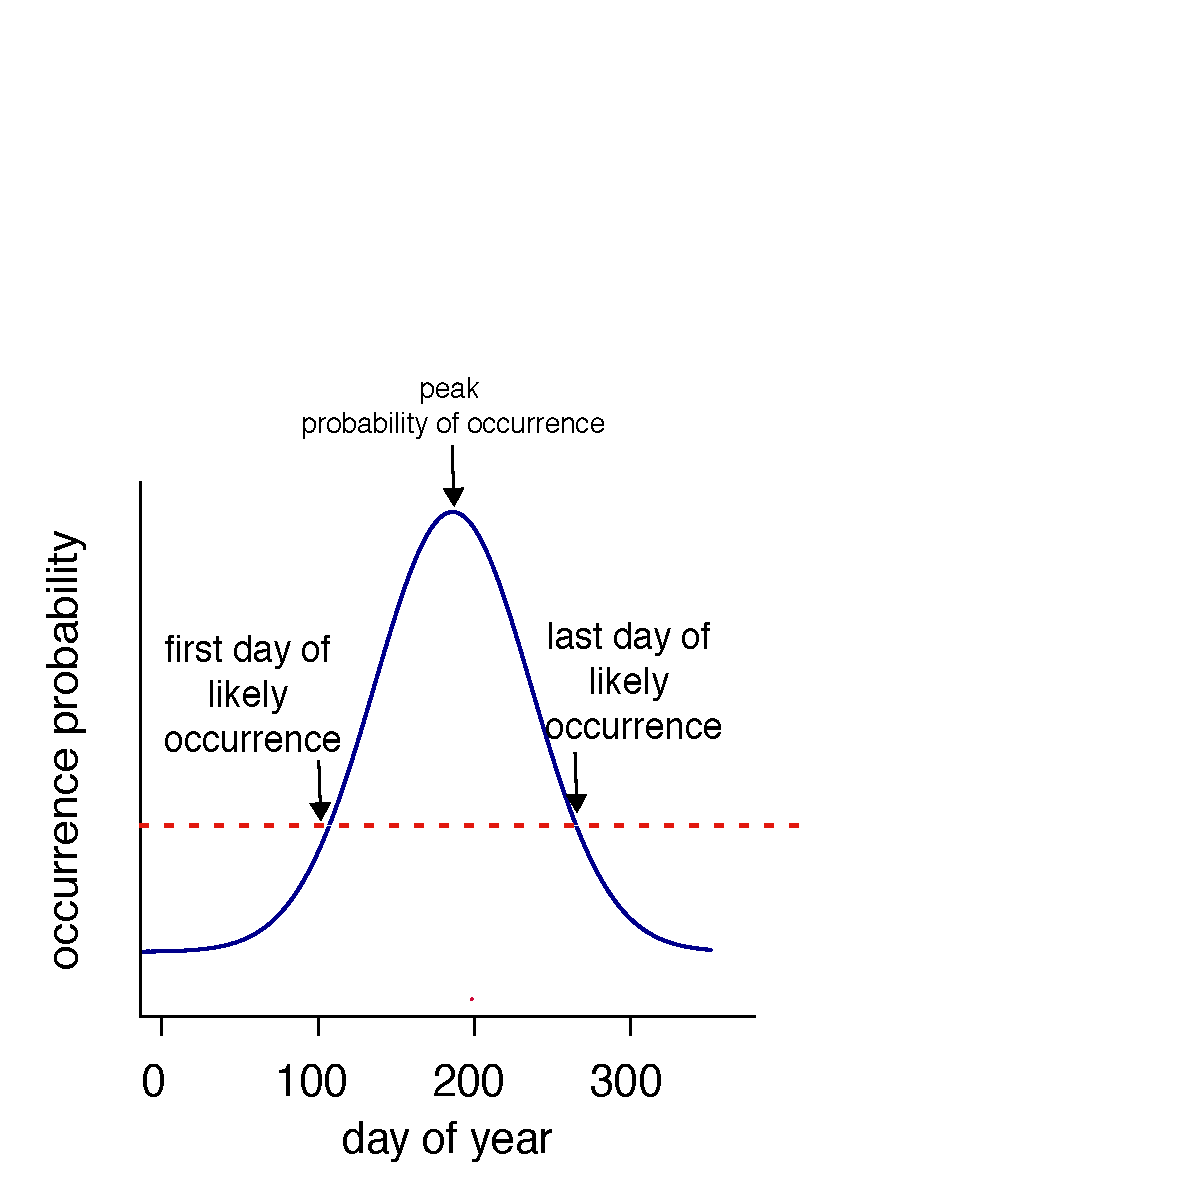
\includegraphics[width=0.7\textwidth]{../analyses/figures/phenophases.pdf}
\caption{\textbf{The phenophases quantified in this study} included day of year of first and last occurrence, as well as day of year of peak occurrence probability for southern resident killer whales and peak abundance index for salmon.}
\label{fig:ctcalb}
\end{figure}

\vspace*{\floatsep}

\begin{figure}[!hp]
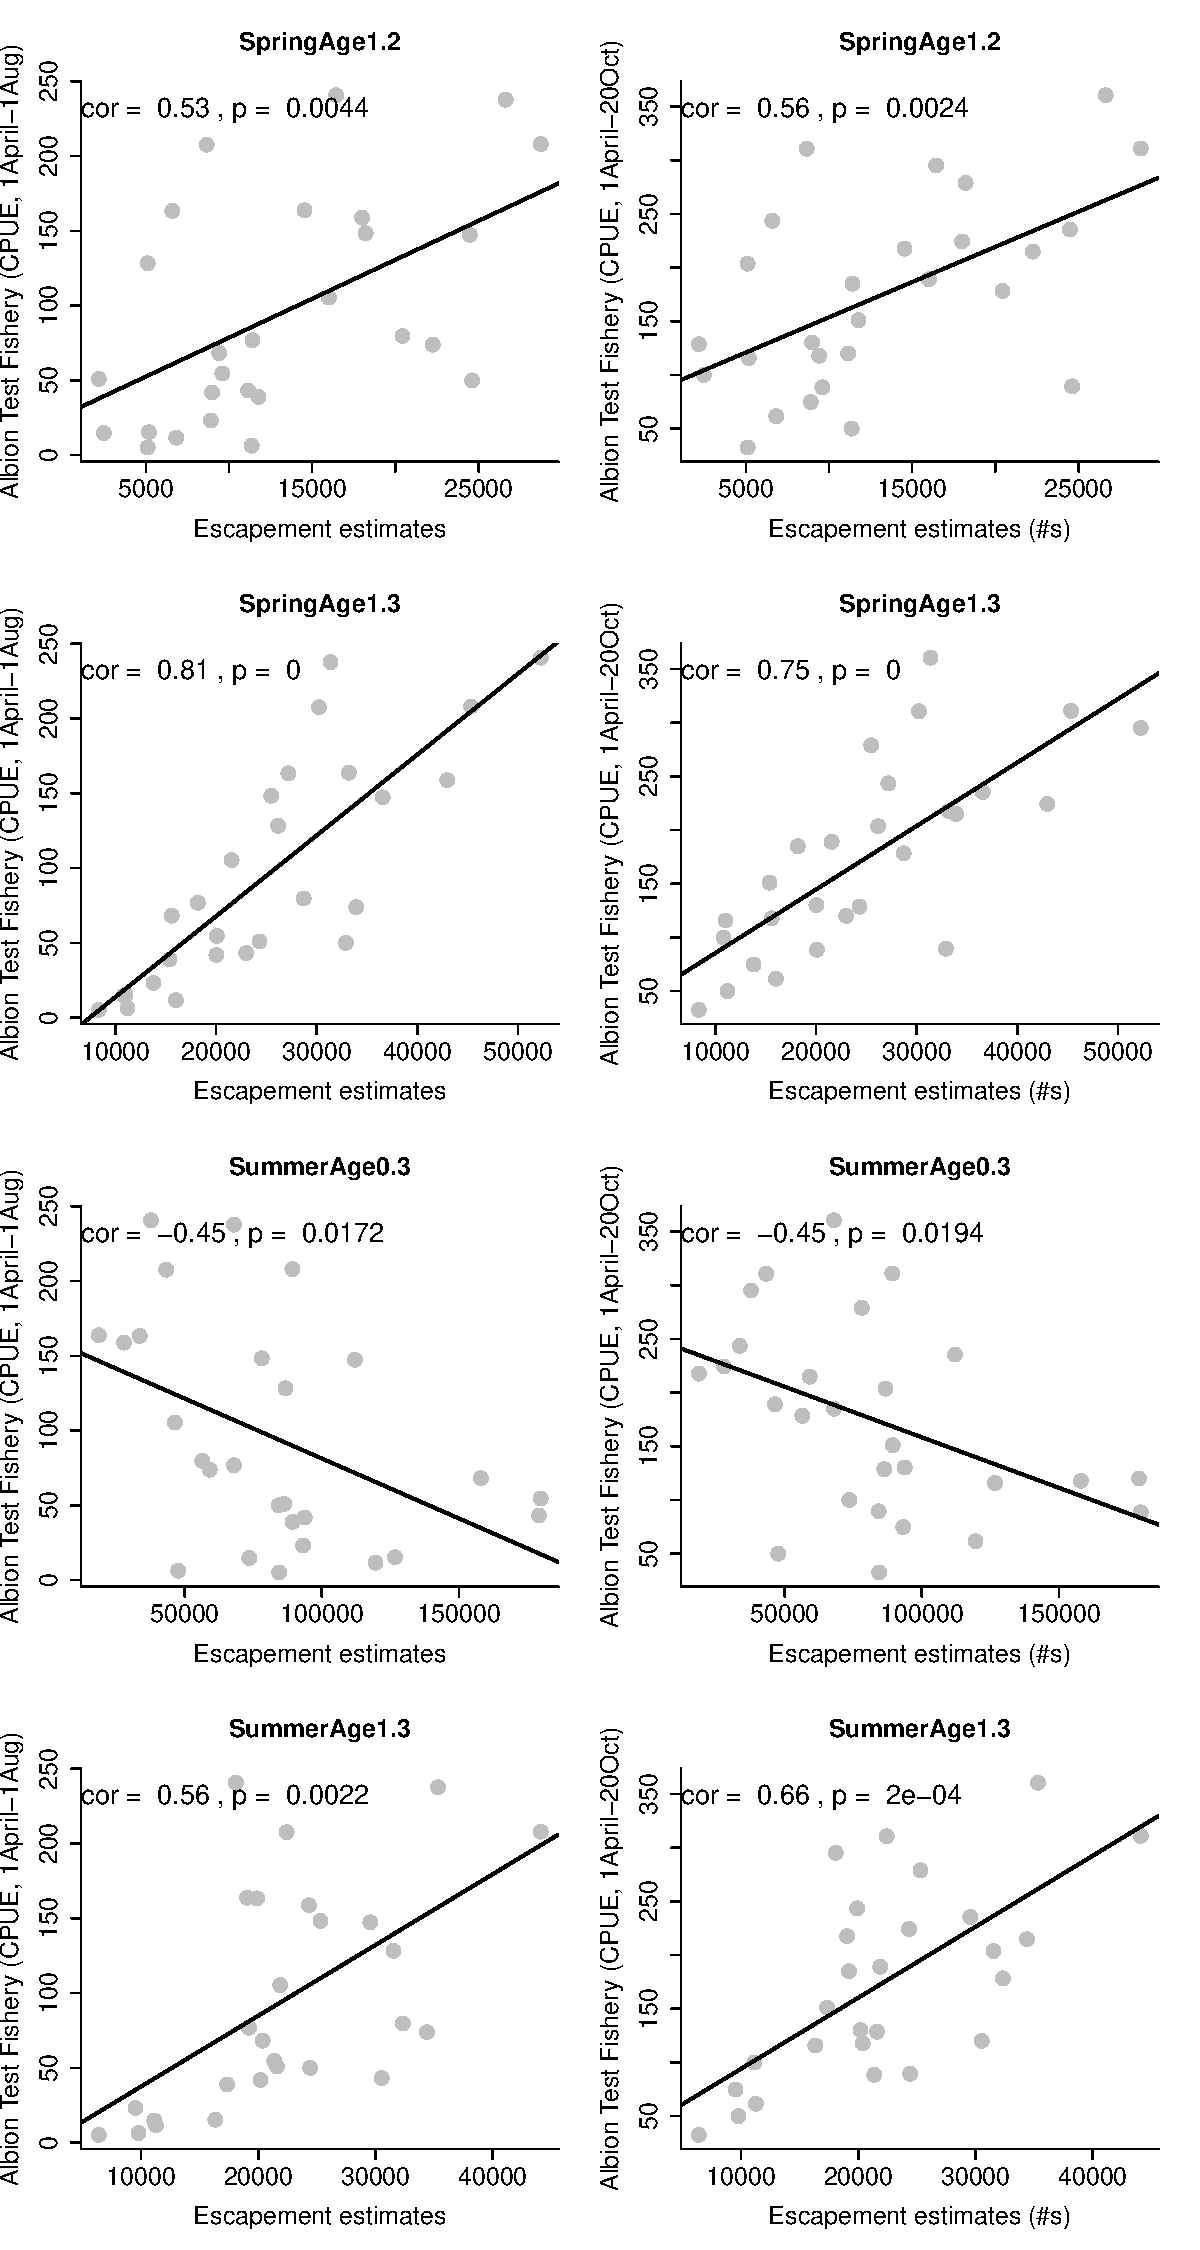
\includegraphics[width=0.7\textwidth]{../analyses/orcaphen/figures/ctcalbion.pdf}
\caption{\textbf{Comparison of the abundance index from Albion test fishery CPUE (used in this paper) to alternative indices of abundance: total escapement from four index stocks used by the Pacific Salmon Commission (PSC 2018)}, from 1975-2018. Top row shows relationship between Albion Test Fishery CPUE to escapement estimates for four spring and summer index stocks assessed by the Pacific Salmon Commission in the Fraser River: Fraser Spring-Run 1.2, Fraser Spring-Run 1.3, Fraser Summer-Run 1.3, and Fraser Summer Run 0.3.}
\label{fig:ctcalb}
\end{figure}


\vspace*{\floatsep}

\begin{figure}[!hp]
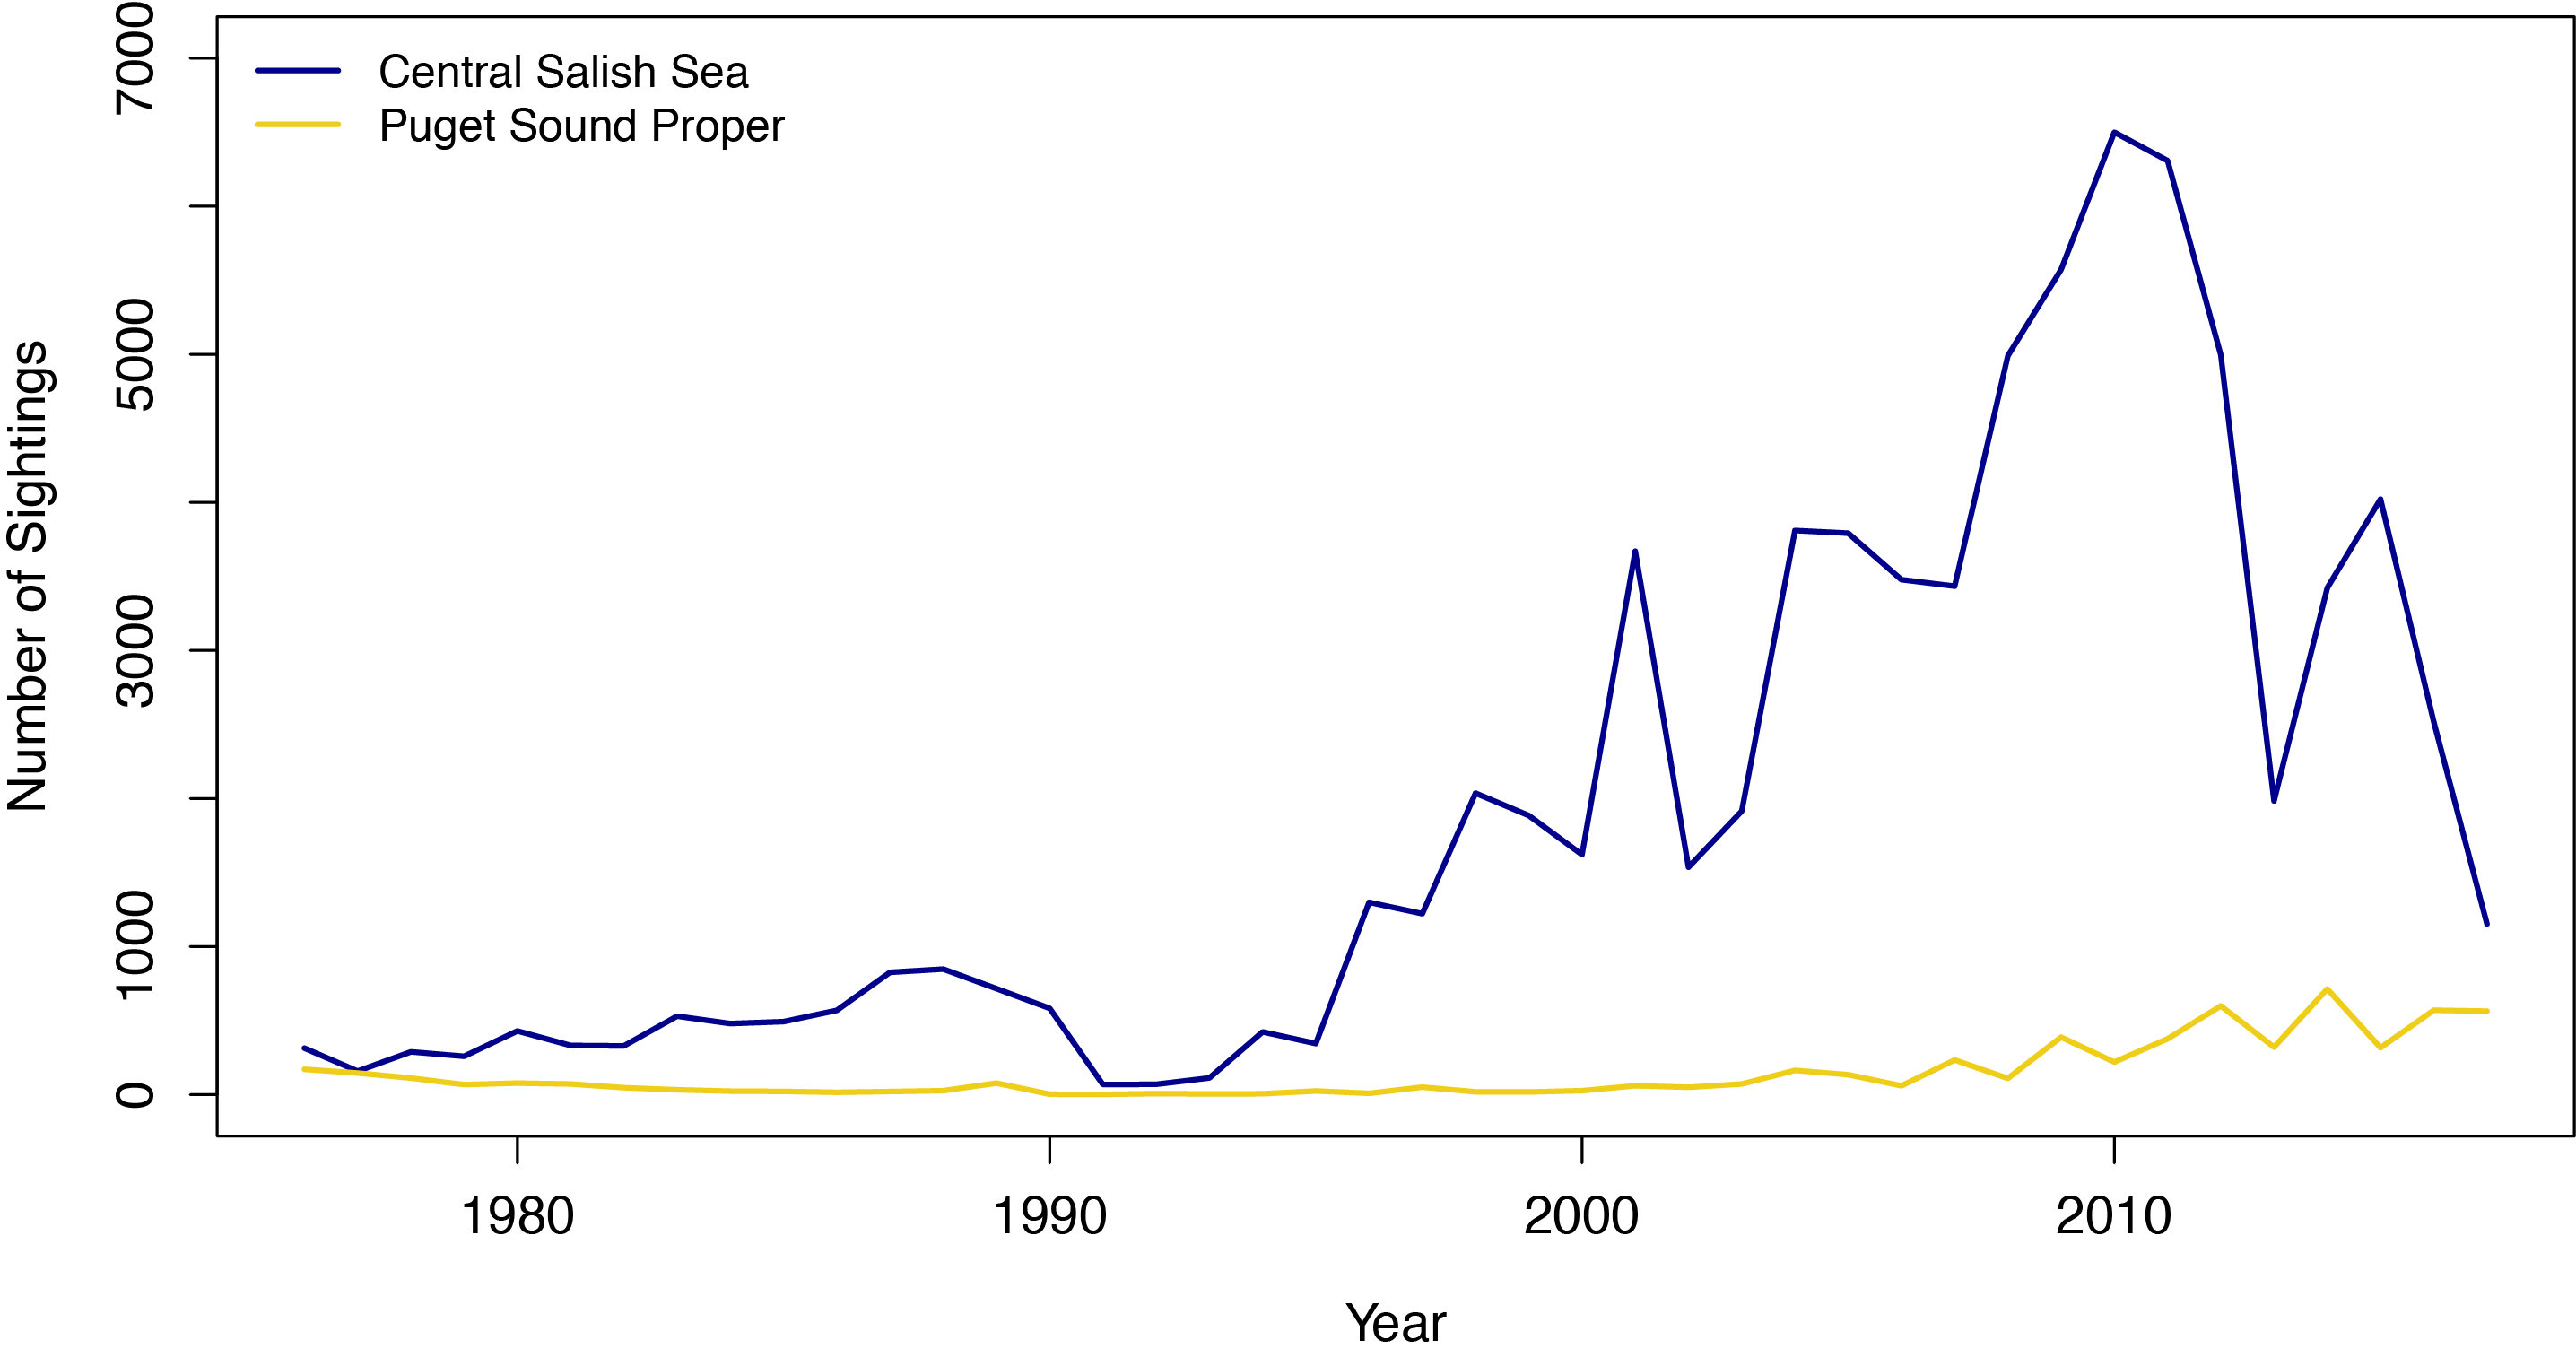
\includegraphics[width=0.8\textwidth]{../analyses/figures/OrcaPhenPlots/numsights_1976_2regs.png} 
\caption{\textbf{Sightings of SRKWs from the Orca Master Database}, from 1978-2017. }
\label{fig:sights}
\end{figure}


\begin{figure}[!hp]
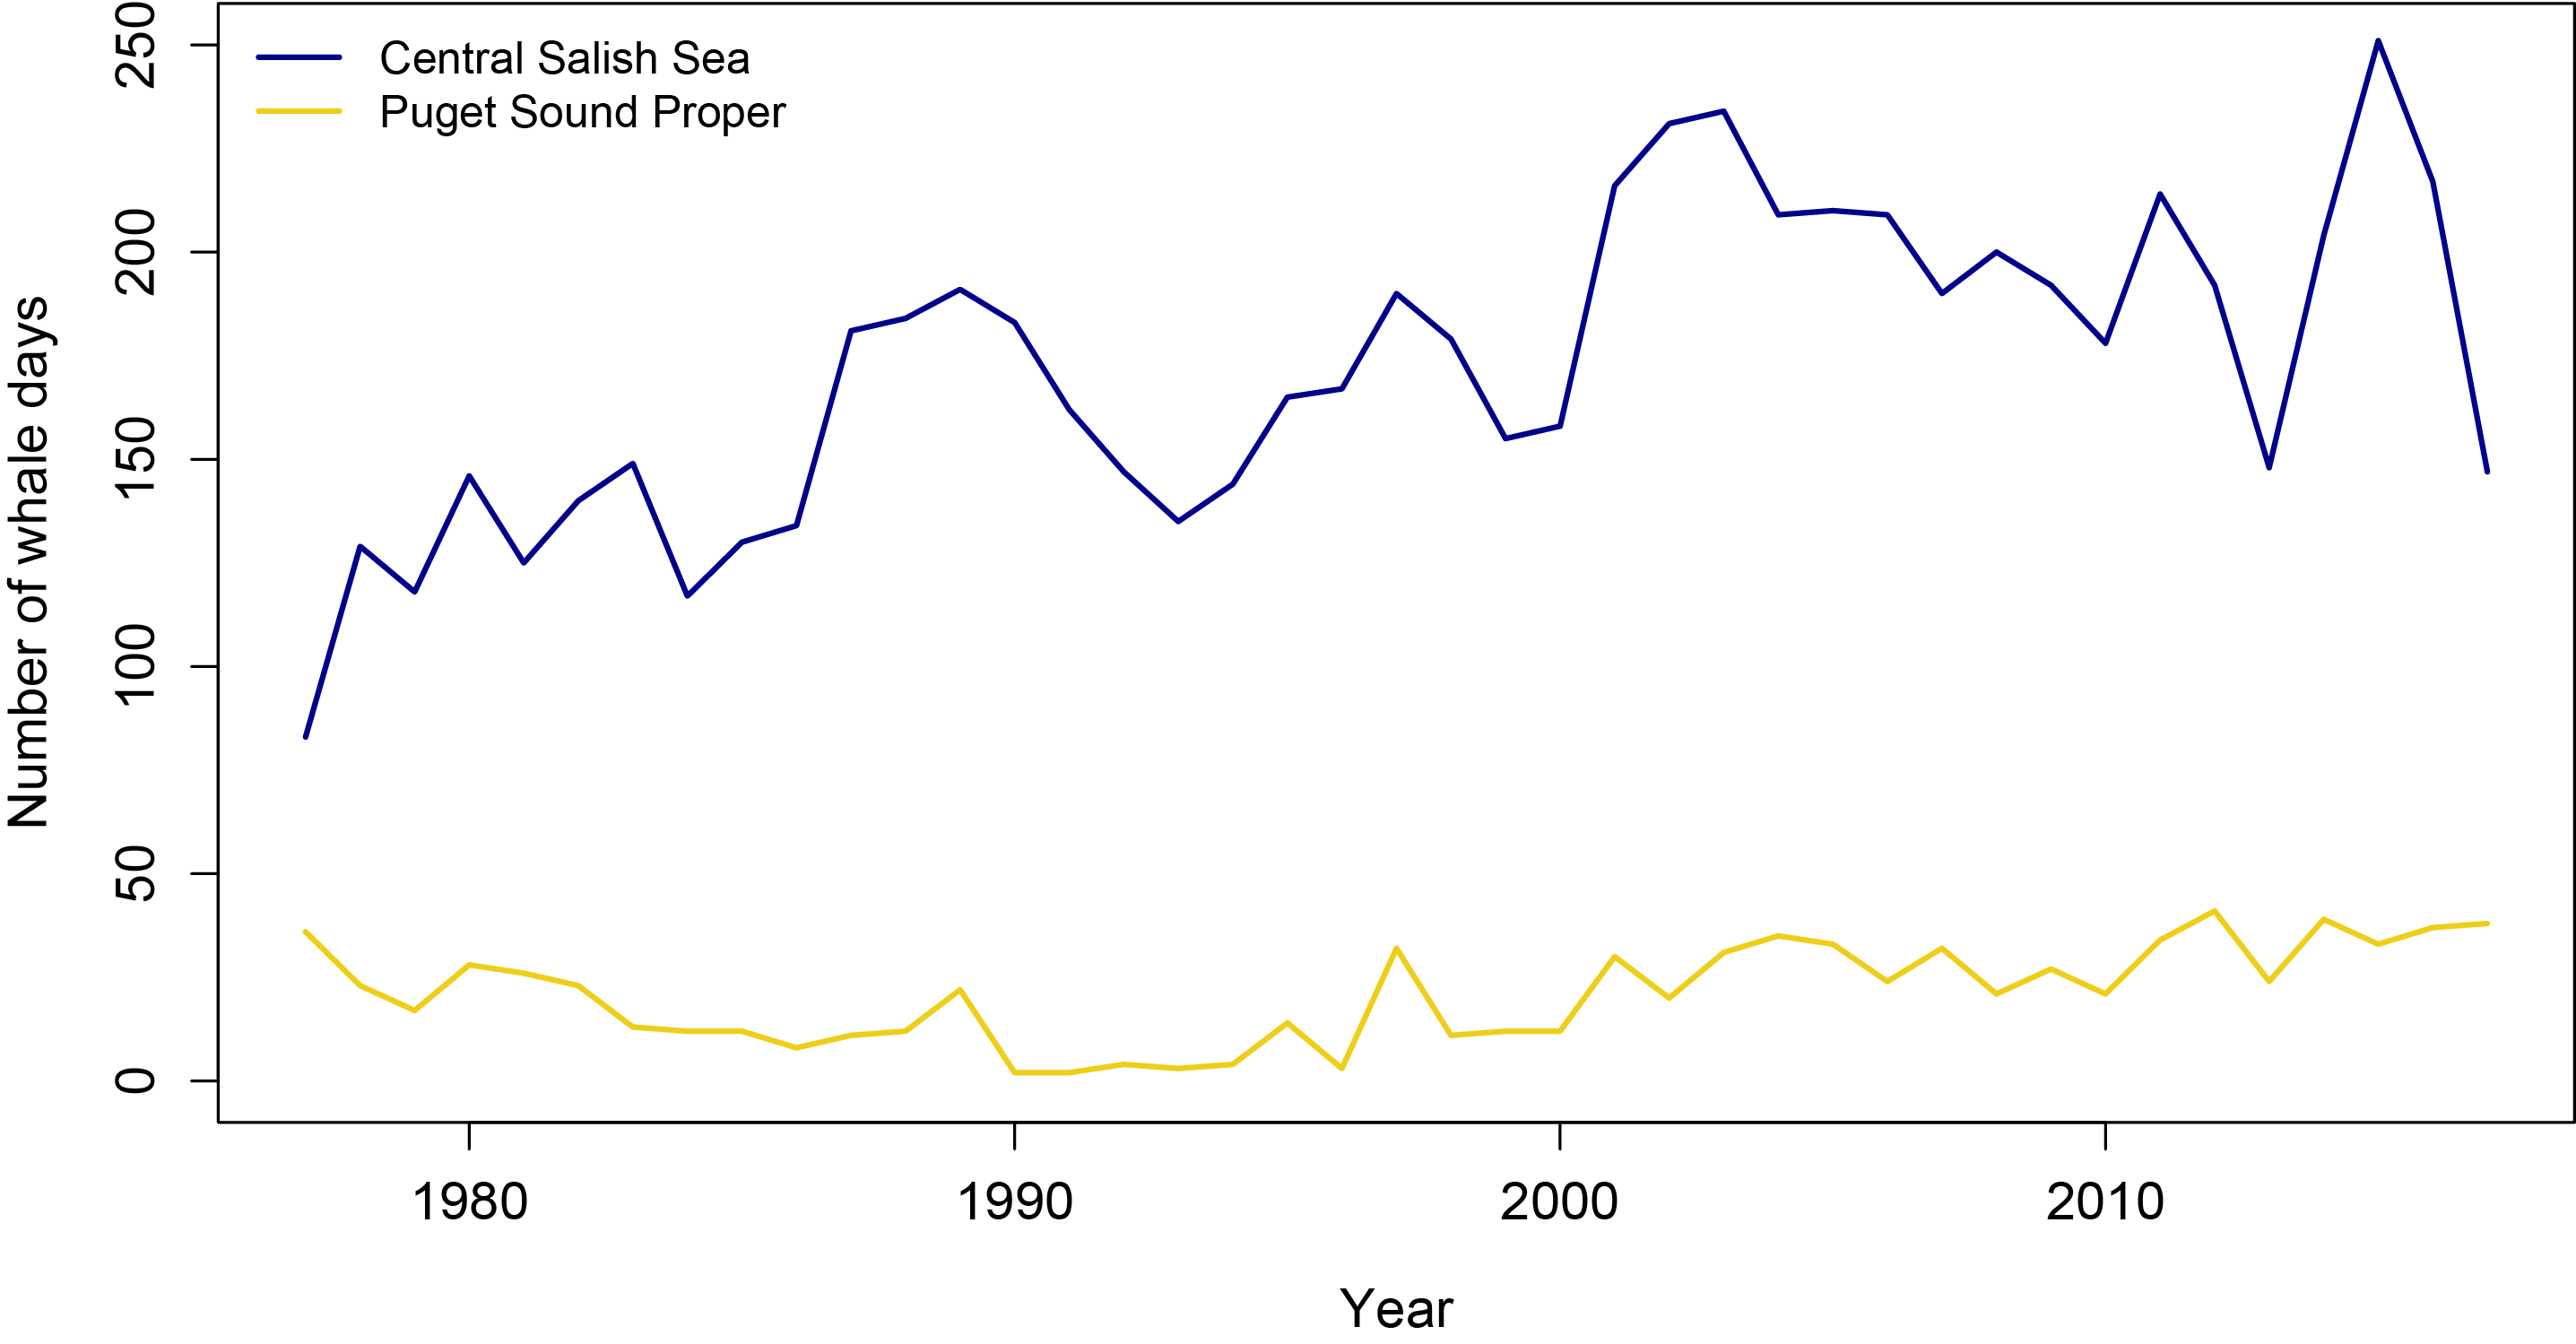
\includegraphics[width=0.8\textwidth]{../analyses/figures/OrcaPhenPlots/whaledays_assumeSRKW2regs.png} 
\caption{\textbf{Number of whale days from the Orca Master Database}, from 1978-2017. }
\label{fig:wdays}
\end{figure}


\begin{figure}[!hp]
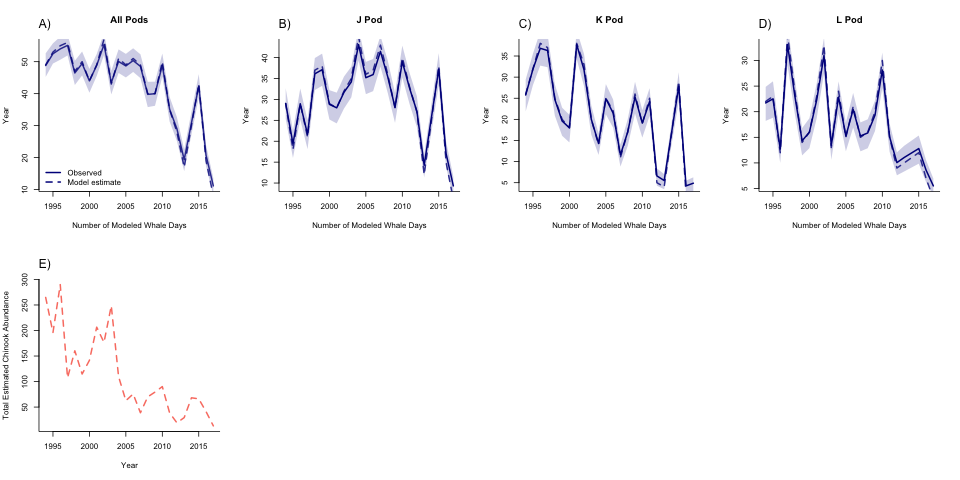
\includegraphics[width=0.8\textwidth]{../analyses/orcaphen/figures/modwhaledays_lime.png} 
\caption{\textbf{Whale days and estimated Chinook abundance have declined at Lime Kiln State Park} since 1994. We show observed and modeled numbers of whale days from our Lime Kiln occupancy model, across all pods (A), J pod (B), K pod (C), and L pod (D), as well as estimated annual catch per unit effort (CPUE, catch per thousand fathom minutes), from our abundance index model fit to Albion test fishery data from May though September across all Chinook. Shading shows 75th percentile uncertainty intervals.}
\label{fig:mlimewdays}
 \end{figure}
 
% \begin{figure}[!hp]
% 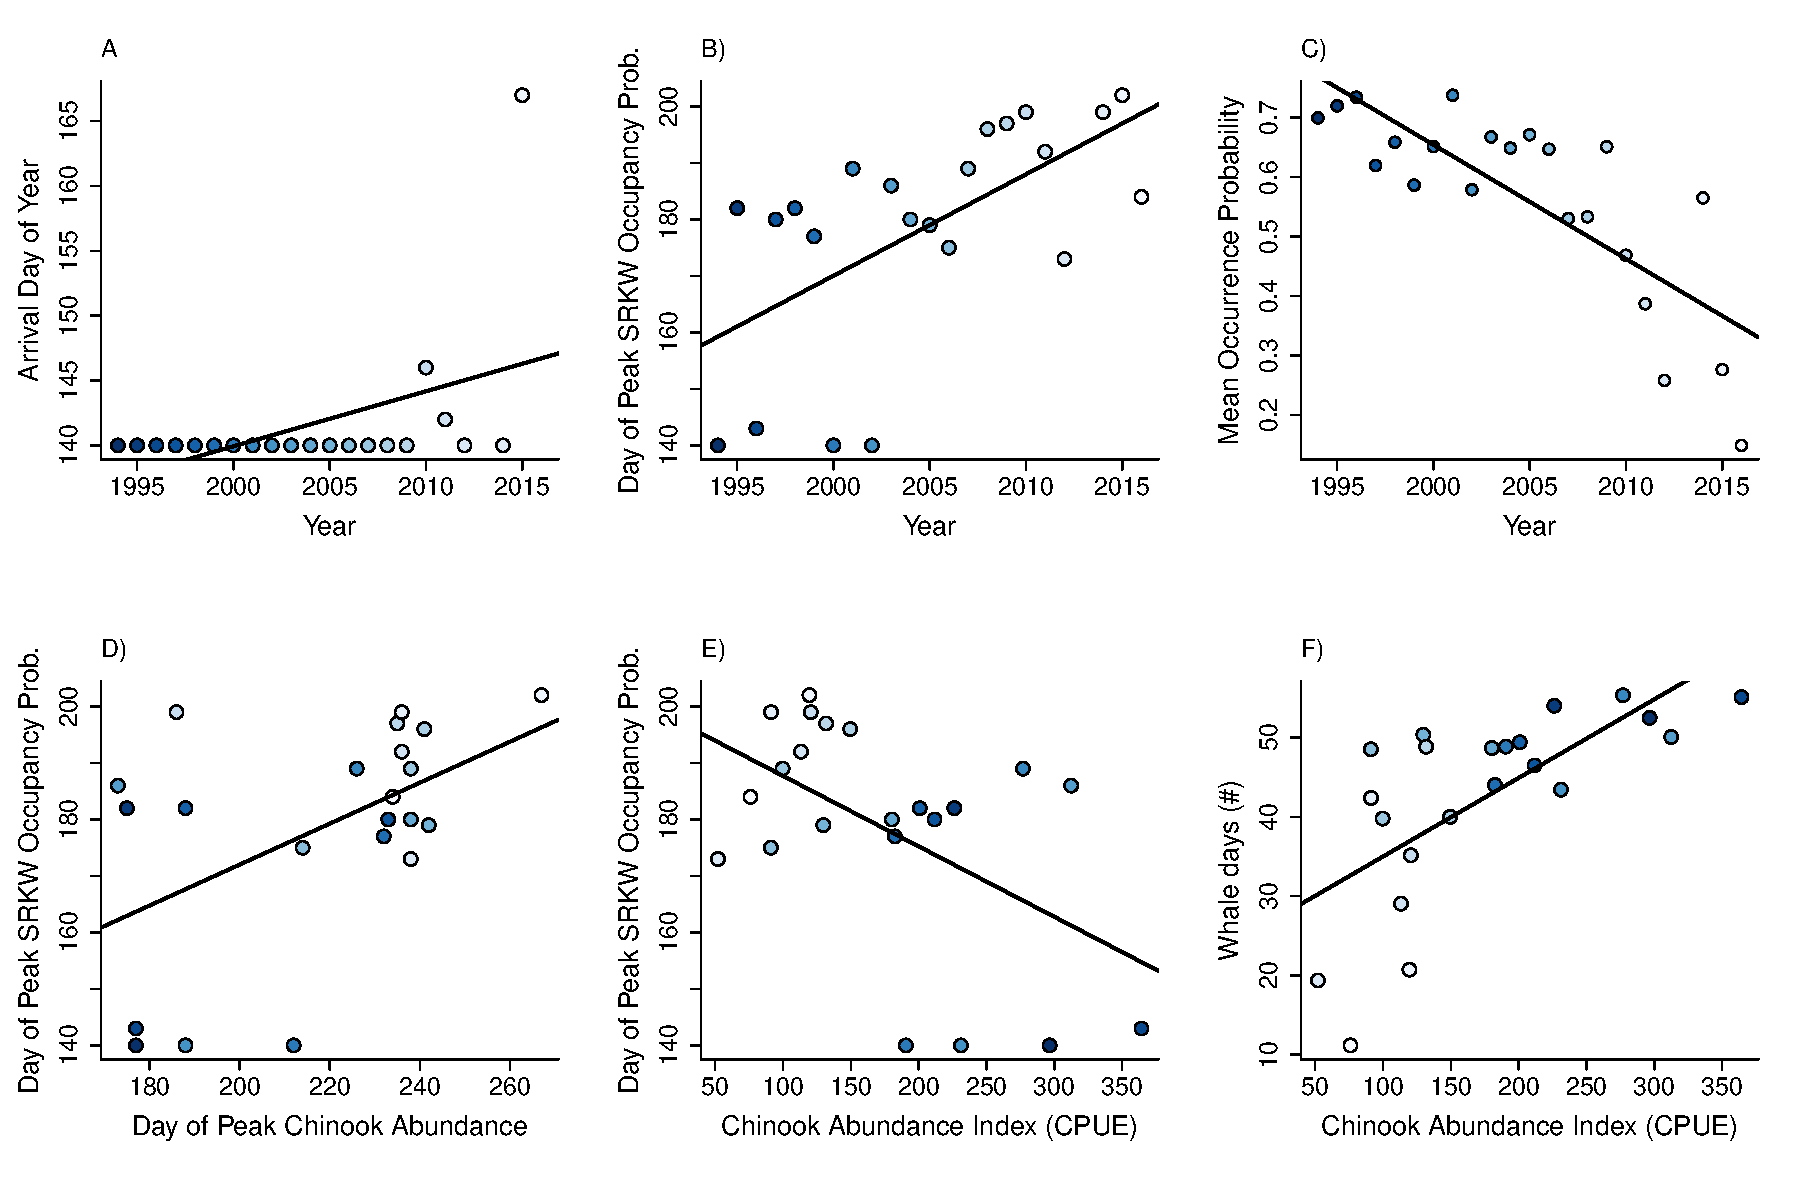
\includegraphics[width=0.99\textwidth]{../analyses/orcaphen/figures/phentrends_lime_peak.pdf} 
% \caption{\textbf{SRKW phenology at Lime Kiln State Park is shifting}, with the likely arrival day of year (A, defined here as the first day of year when the occurrence probability is >0.20) and peak occurrence probability day of year (B) getting later, from 1994-2017. In addition, mean occurrence probability from May to August (the season when regular monitoring of SRKWs occurs at Lime Kiln) is declining during this time period (C). These trends are associated with a decrease in the amount of time SRKWs are spending near Lime Kiln (i.e., the number of days on which SRKWs were observed ("whale days") has declined since 1994 (Fig. \ref{fig:mlimewdays}) and are consistent with shifts in the timing of peak abundance (D) and abundance index (E,F) of their preferred prey, Fraser River Chinook Salmon. (See also Fig. 3 in the main text).}
% \label{fig:limetime}
% \end{figure}

\newpage
\begin{figure}[!hp]
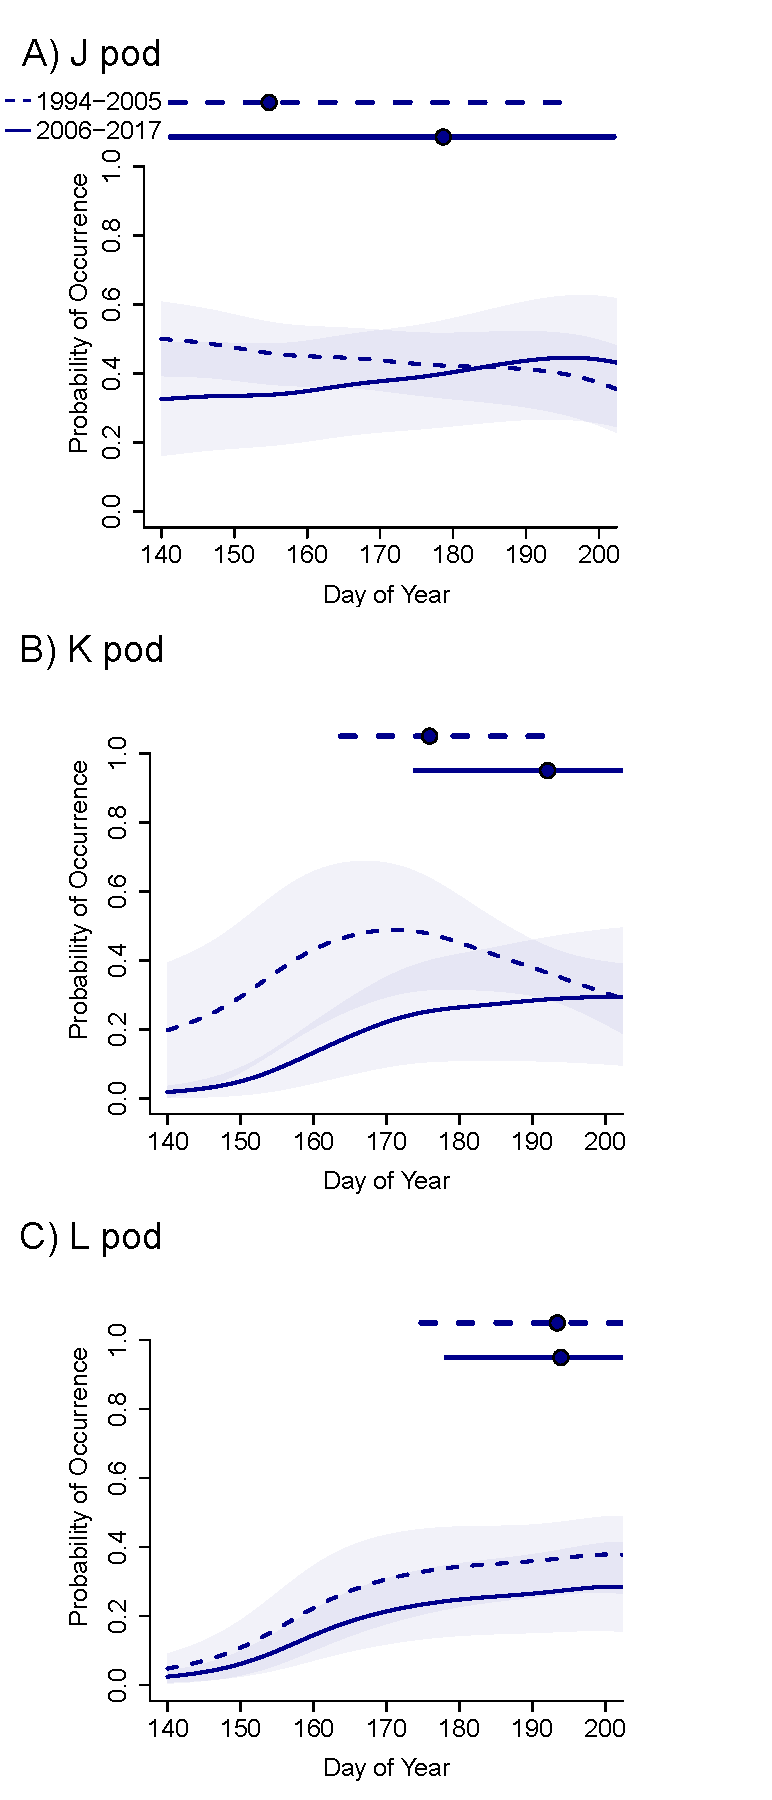
\includegraphics[width=0.5\textwidth]{../analyses/orcaphen/figures/orcachinphenoverlap_allpods2006.pdf}
\caption{\textbf{SRKW phenology has shifted, in concert with shifts in Fraser River Chinook Salmon at one site with consistent observations in the Central Salish Sea}. Phenology (blue lines) is quantified from Lime Kiln Point State Park, SRKW phenology has shifted, with peak arrival dates delaying in recent (solid lines) compared with earlier (dashed lines) years. We show patterns for J-pod (A), K-pod (B), and L-Pod (C). Compare to Fig. 3A of the main text, which shows all pods together. }
\label{fig:KLchin}
\end{figure}

\newpage
\begin{figure}[!hp]
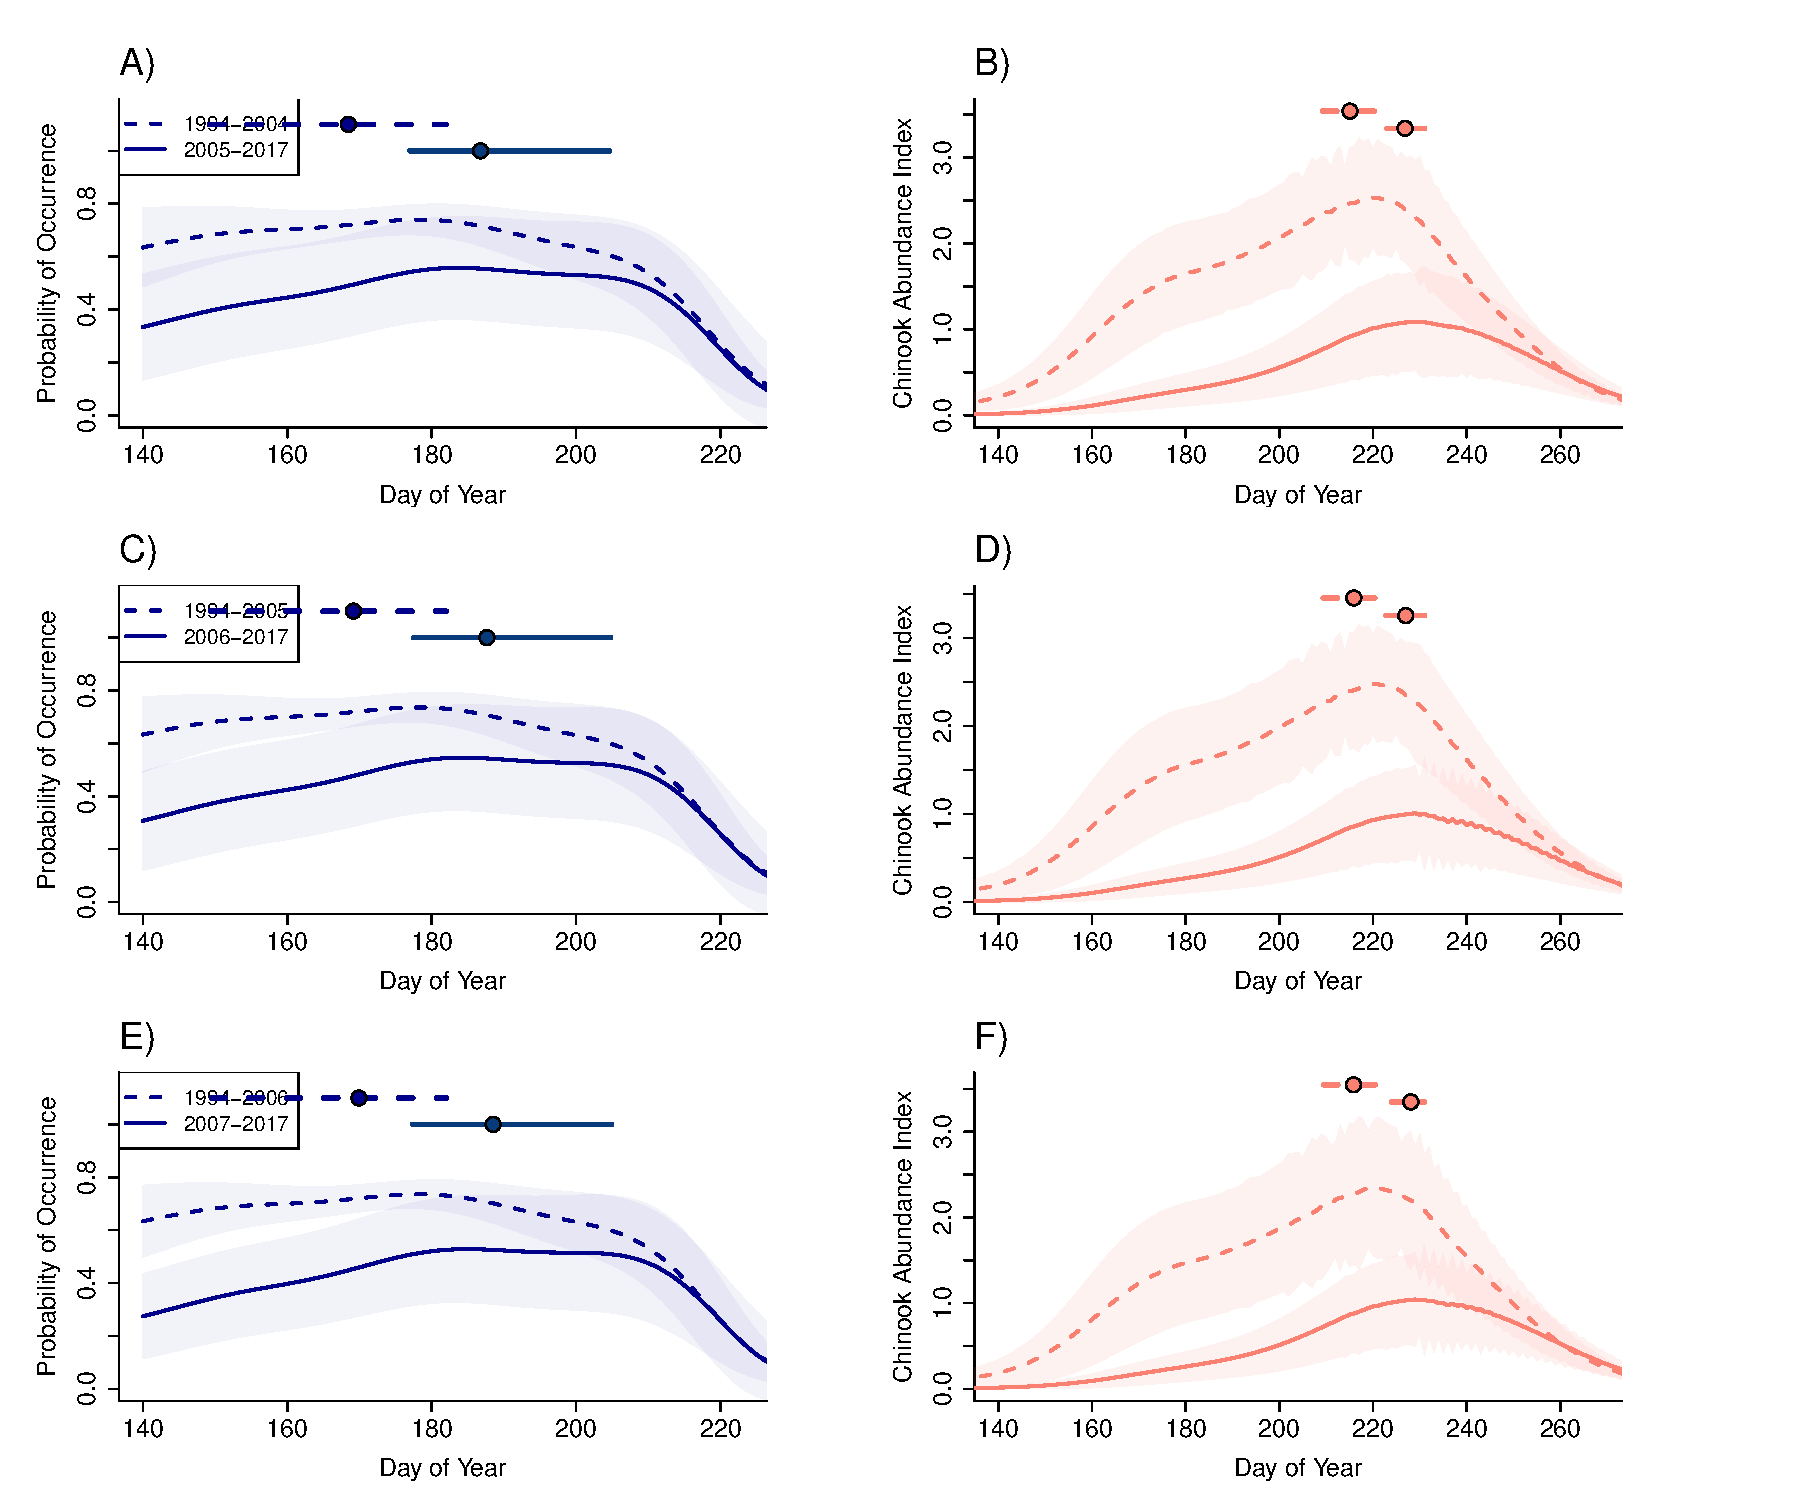
\includegraphics[width=0.9\textwidth]{../analyses/orcaphen/figures/orcachinphenoverlapbrmsSRallbrkyears.pdf}
\caption{\textbf{Changing the break-point has little qualitative effect on patterns of shifts in SRKW and Fraser River Chinook phenology}. We show patterns for all SRKW pods together (as in Figure 3 in the main text) with different breakpoints of 2005 (A,B), 2006 (C,D, as in Fig. 3-4 in main text) and 2007 (E,F). SRKW phenology (blue lines, A,C,E) is quantified from Lime Kiln Point State Park; Fraser River Chinook phenology is quantified using the Albion test fishery dataset. An index of adult Fraser River Chinook salmon (summed daily CPUE from this dataset, from April through August, pink lines) and SRKW phenology have shifted, with peak occupancy and abundance dates delaying in recent (solid lines) compared with earlier years (dashed lines).}
\label{fig:brkpt}
\end{figure}


\begin{figure}[!hp]
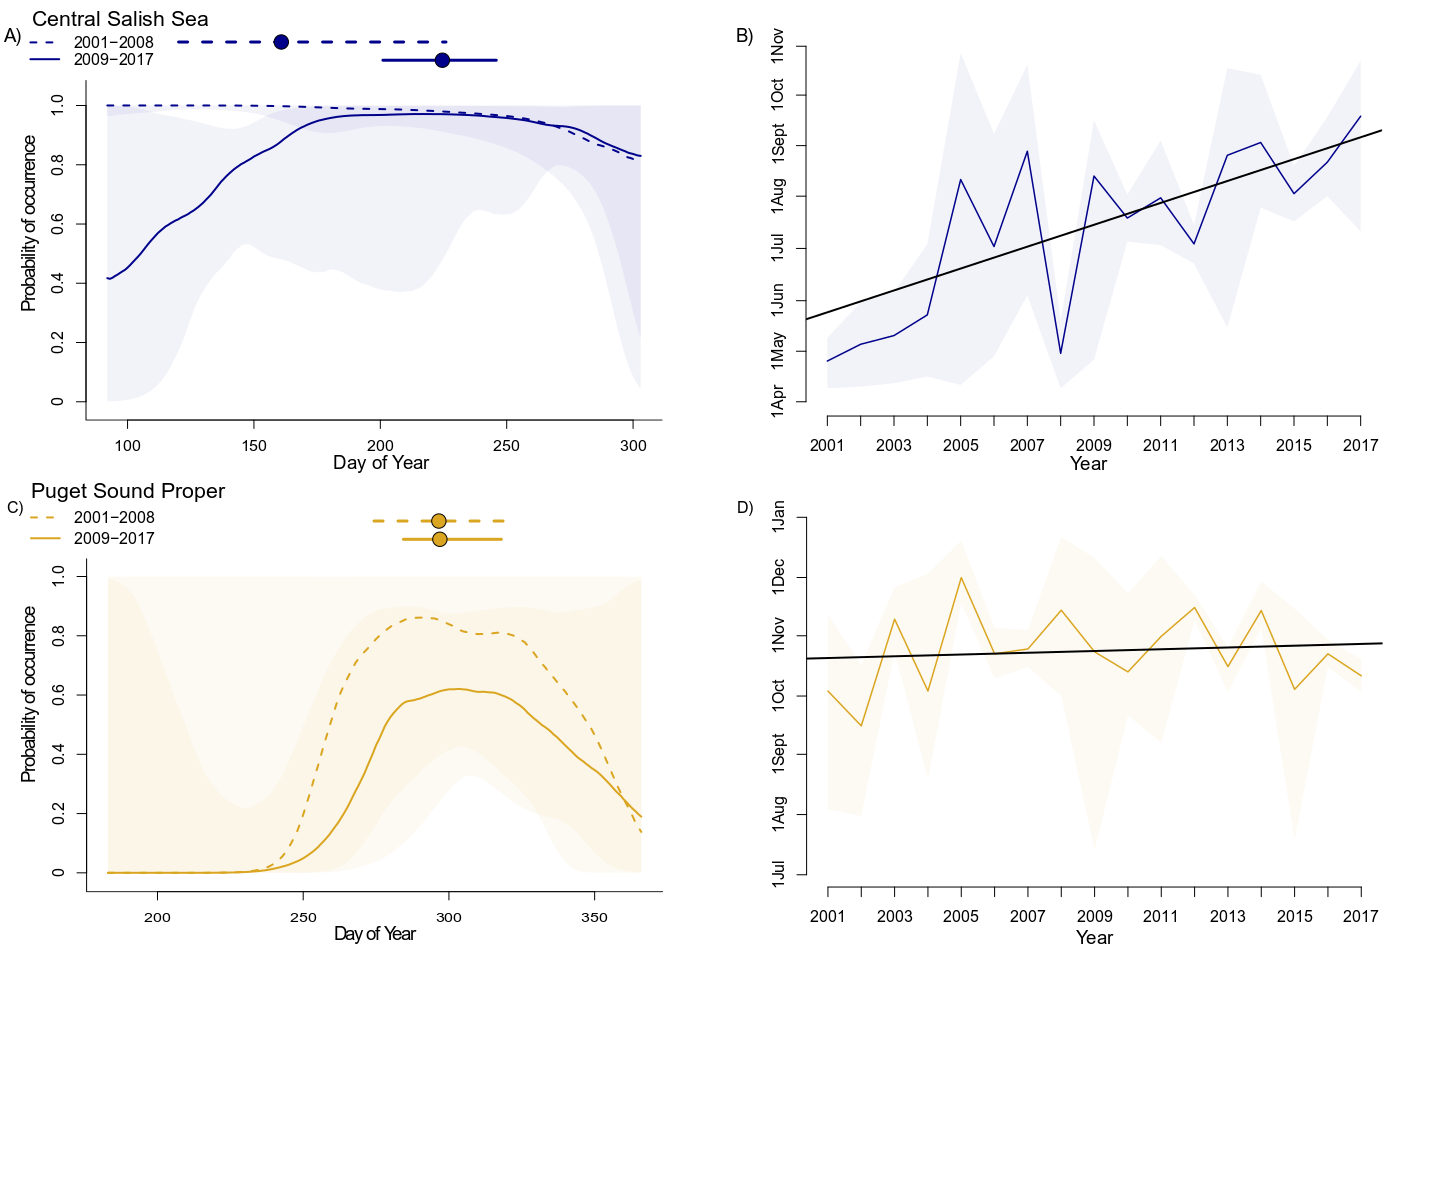
\includegraphics[width=0.8\textwidth]{../analyses/figures/proboccJ_4panels.png} 
\caption{\textbf{J-pod activity varies seasonally in the Central Salish Sea (A) and Puget Sound proper (C).} This phenology has shifted later in recent years in the Central Salish Sea (B) and in Puget Sound (D). The shift toward later arrival in the central Salish Sea is evident the estimated probabilities of occurrence from the occupancy models for K-pod (A,C) as well as the linear trends in peak occurrence probability from 2001-2017 (B,D). Shading around lines represents 75\% uncertainty intervals. 
}
\label{fig:Jprobs}
\end{figure}

\begin{figure}[!hp]
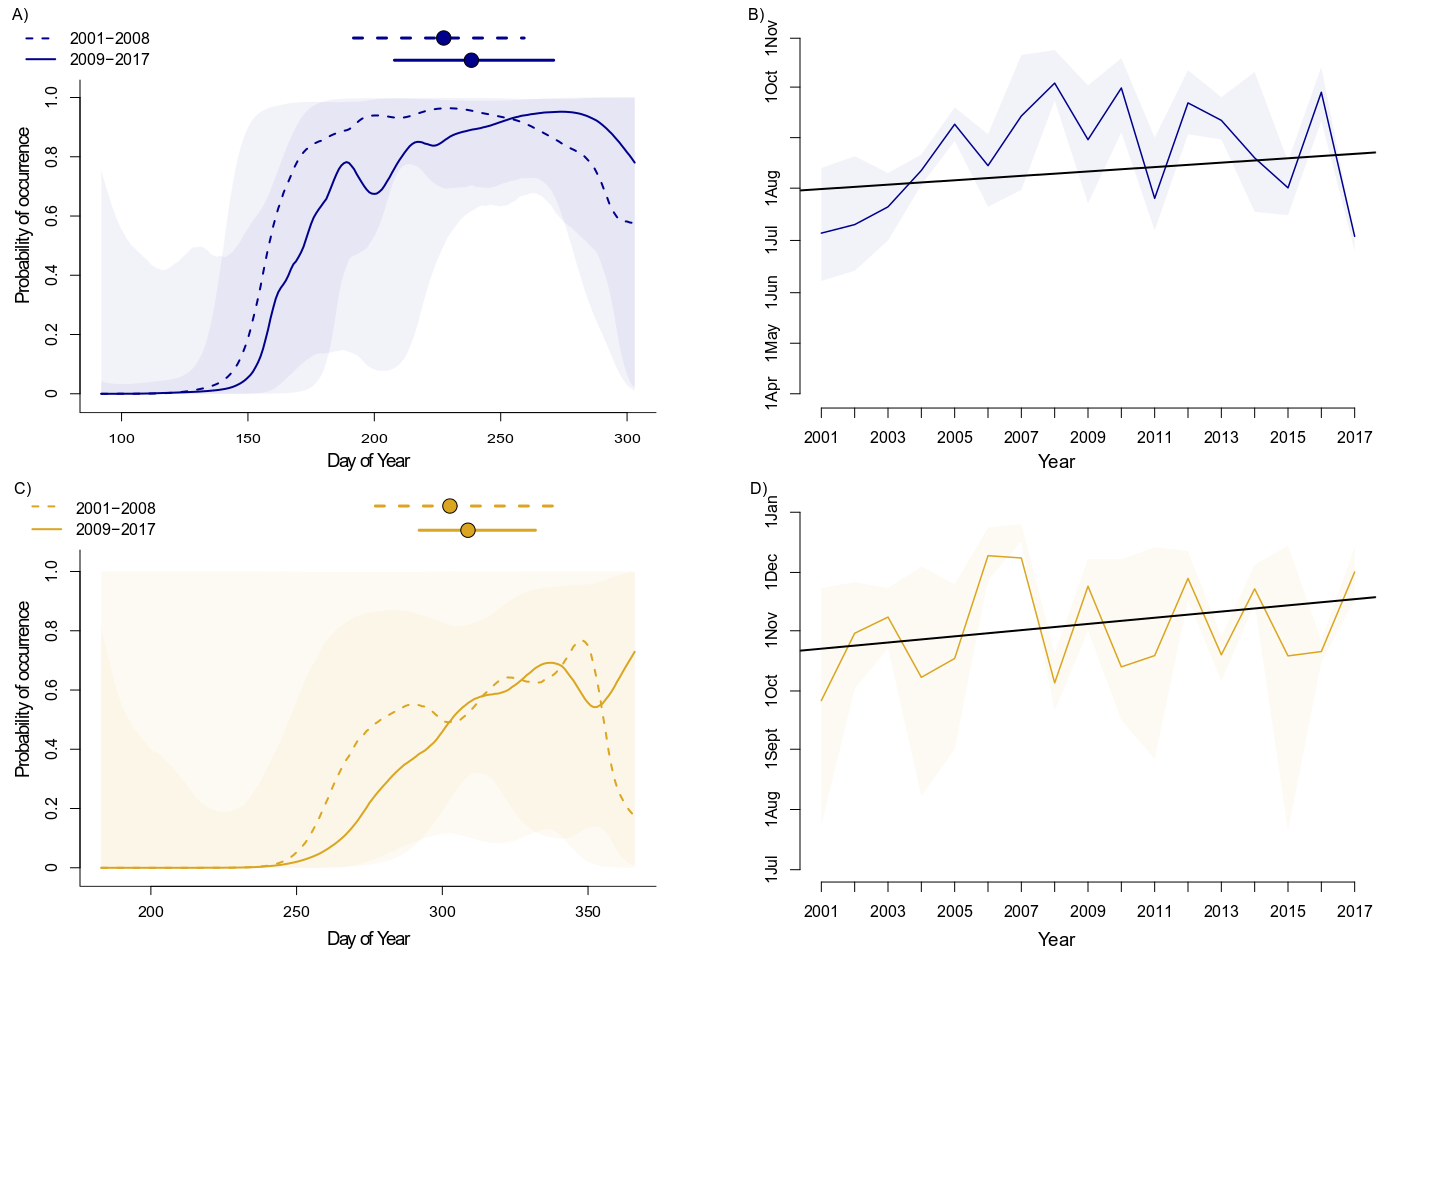
\includegraphics[width=0.8\textwidth]{../analyses/figures/proboccK_4panels.png} 
\caption{\textbf{K-pod activity varies seasonally in the Central Salish Sea (A) and Puget Sound proper (C).} This phenology has shifted later in recent years in the Central Salish Sea (B) and in Puget Sound (D). The shift toward later arrival in the central Salish Sea is evident the estimated probabilities of occurrence from the occupancy models for K-pod (A,C) as well as the linear trends in peak occurrence probability from 2001-2017 (B,D). Shading around lines represents 75\% credible intervals. 
}
\label{fig:Kprobs}
\end{figure}


\begin{figure}[!hp]
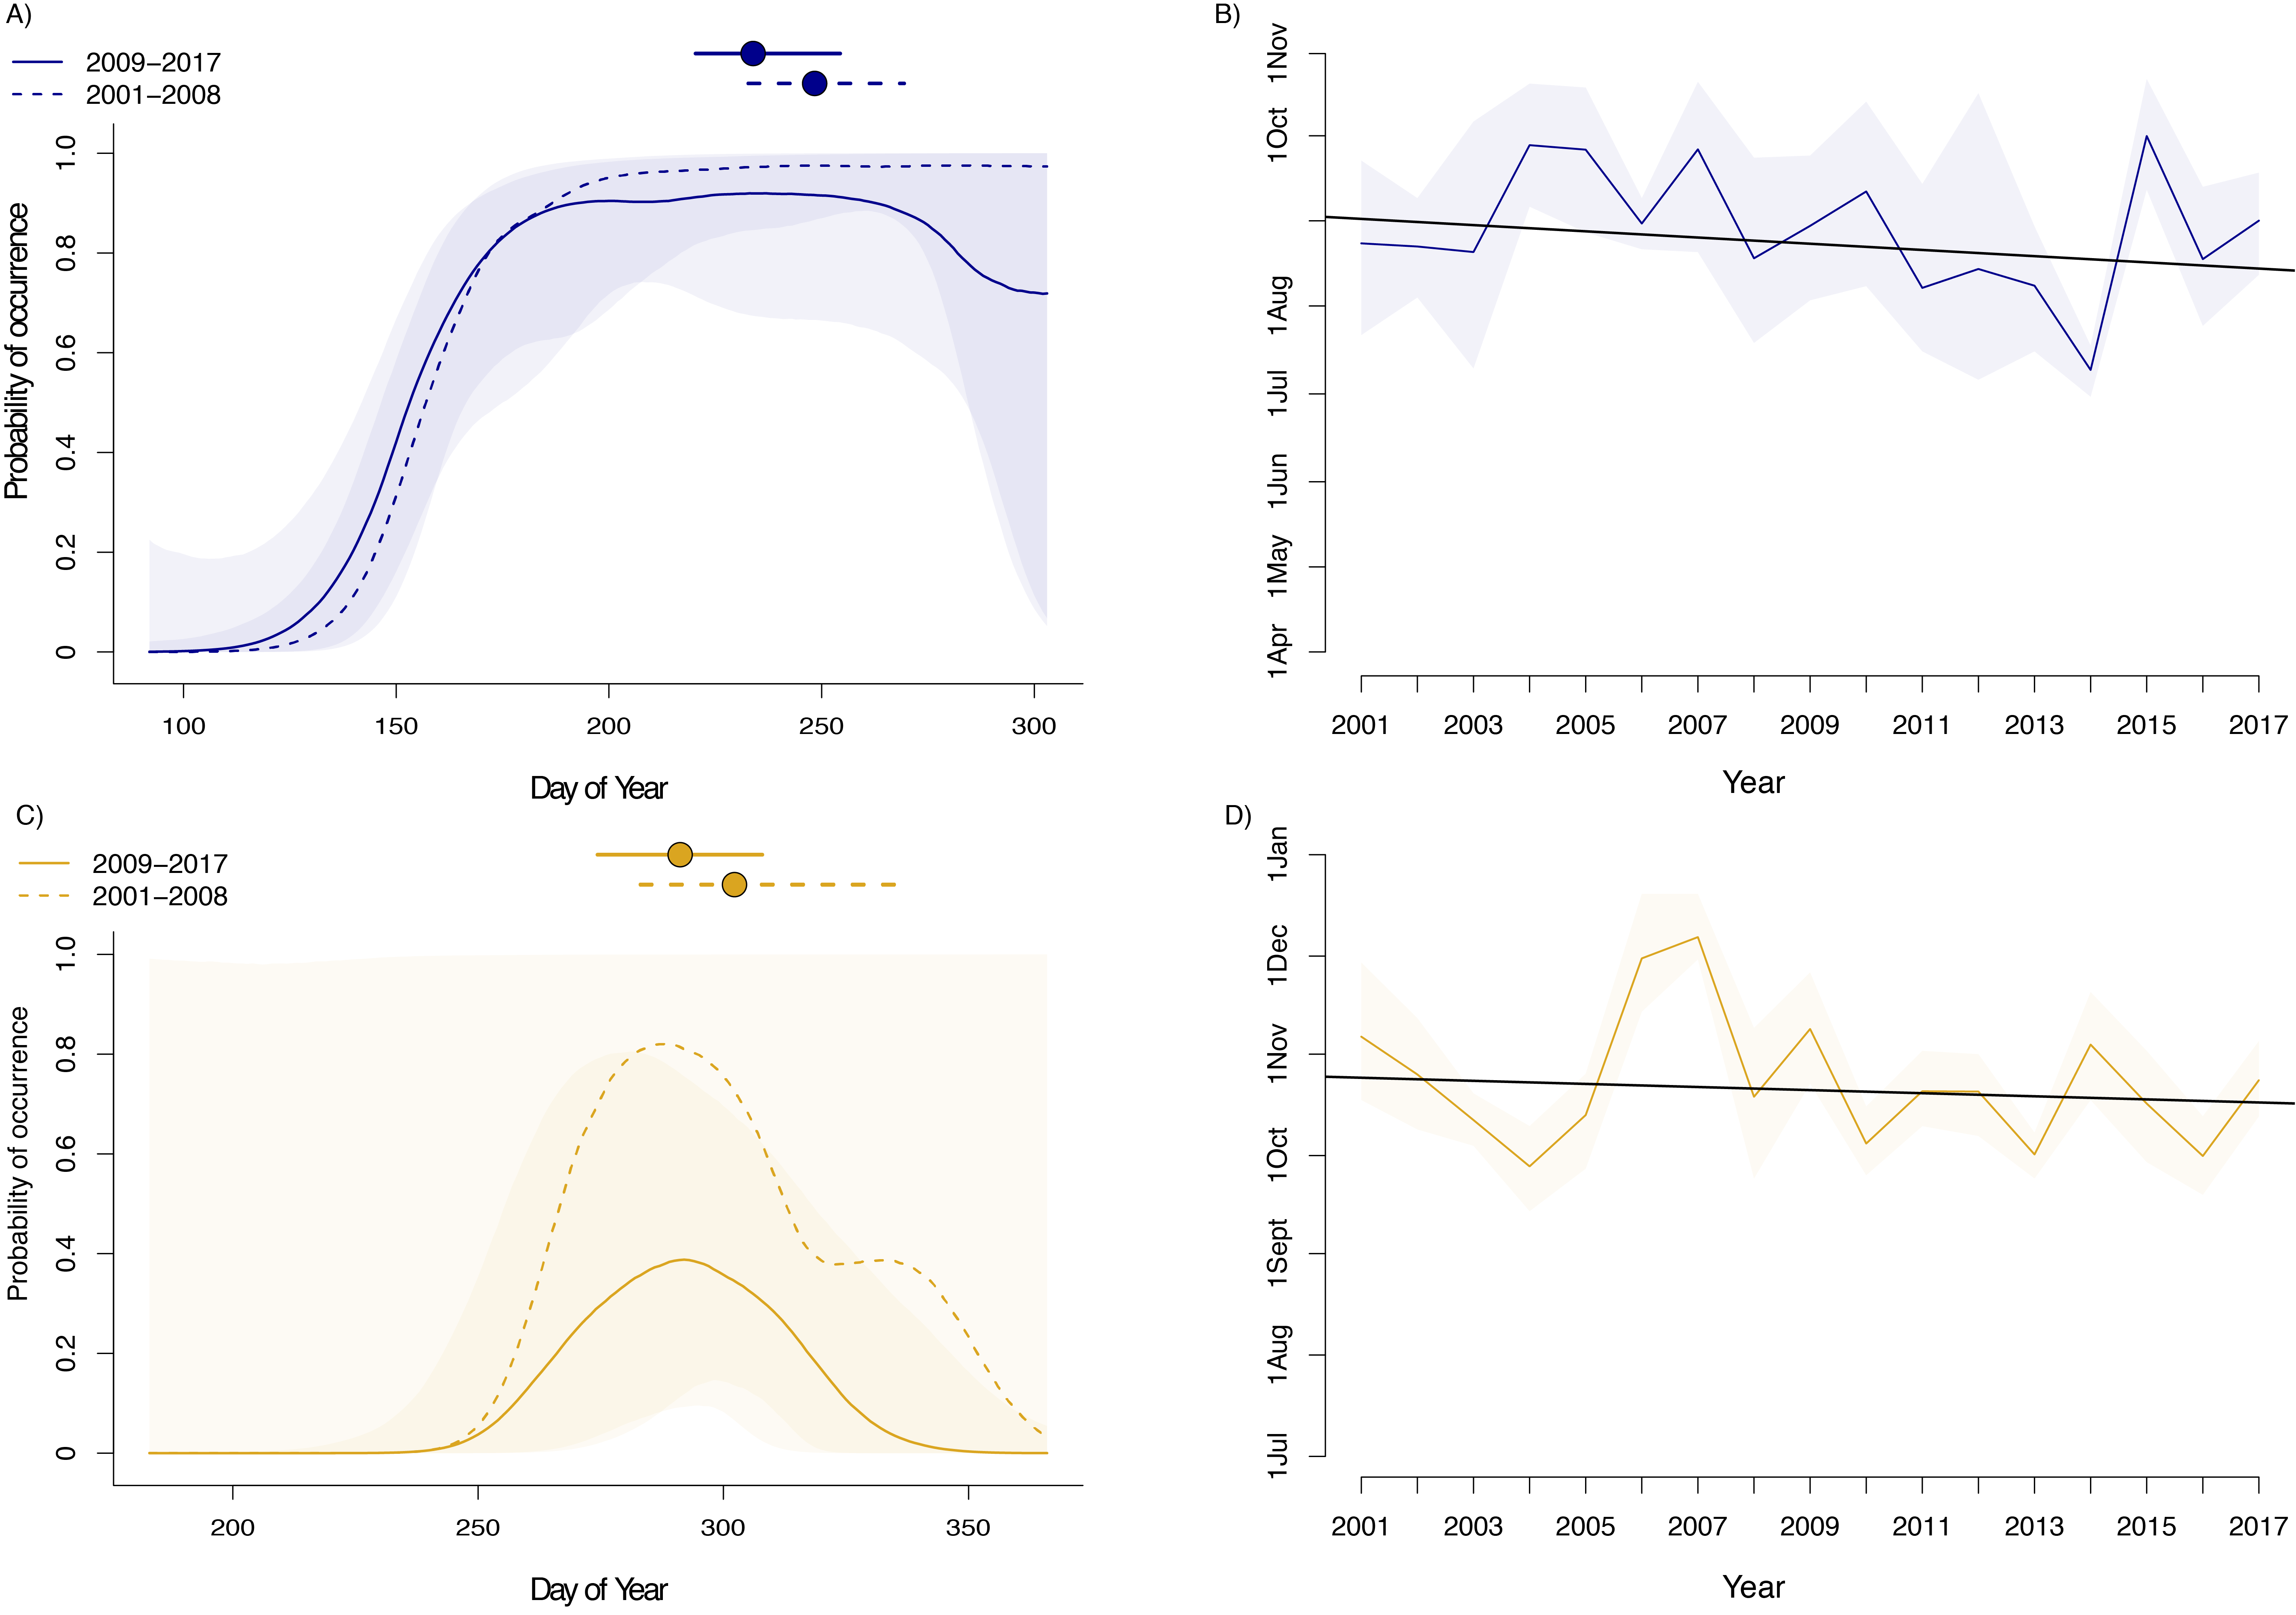
\includegraphics[width=0.8\textwidth]{../analyses/figures/proboccL_4panels.png} 
\caption{\textbf{L-pod activity varies seasonally in the Central Salish Sea (A) and Puget Sound proper (C)}. This phenology has shifted later in recent years in the Central Salish Sea (B) and in Puget Sound (D). The shift toward later arrival in the central Salish Sea is evident the estimated probabilities of occurrence from the occupancy models for K-pod (A,C) as well as the linear trends in peak occurrence probability from 2001-2017 (B,D). Shading around lines represents 75\% credible intervals. 
}
\label{fig:Lprobs}
\end{figure}

\begin{figure}[!hp]
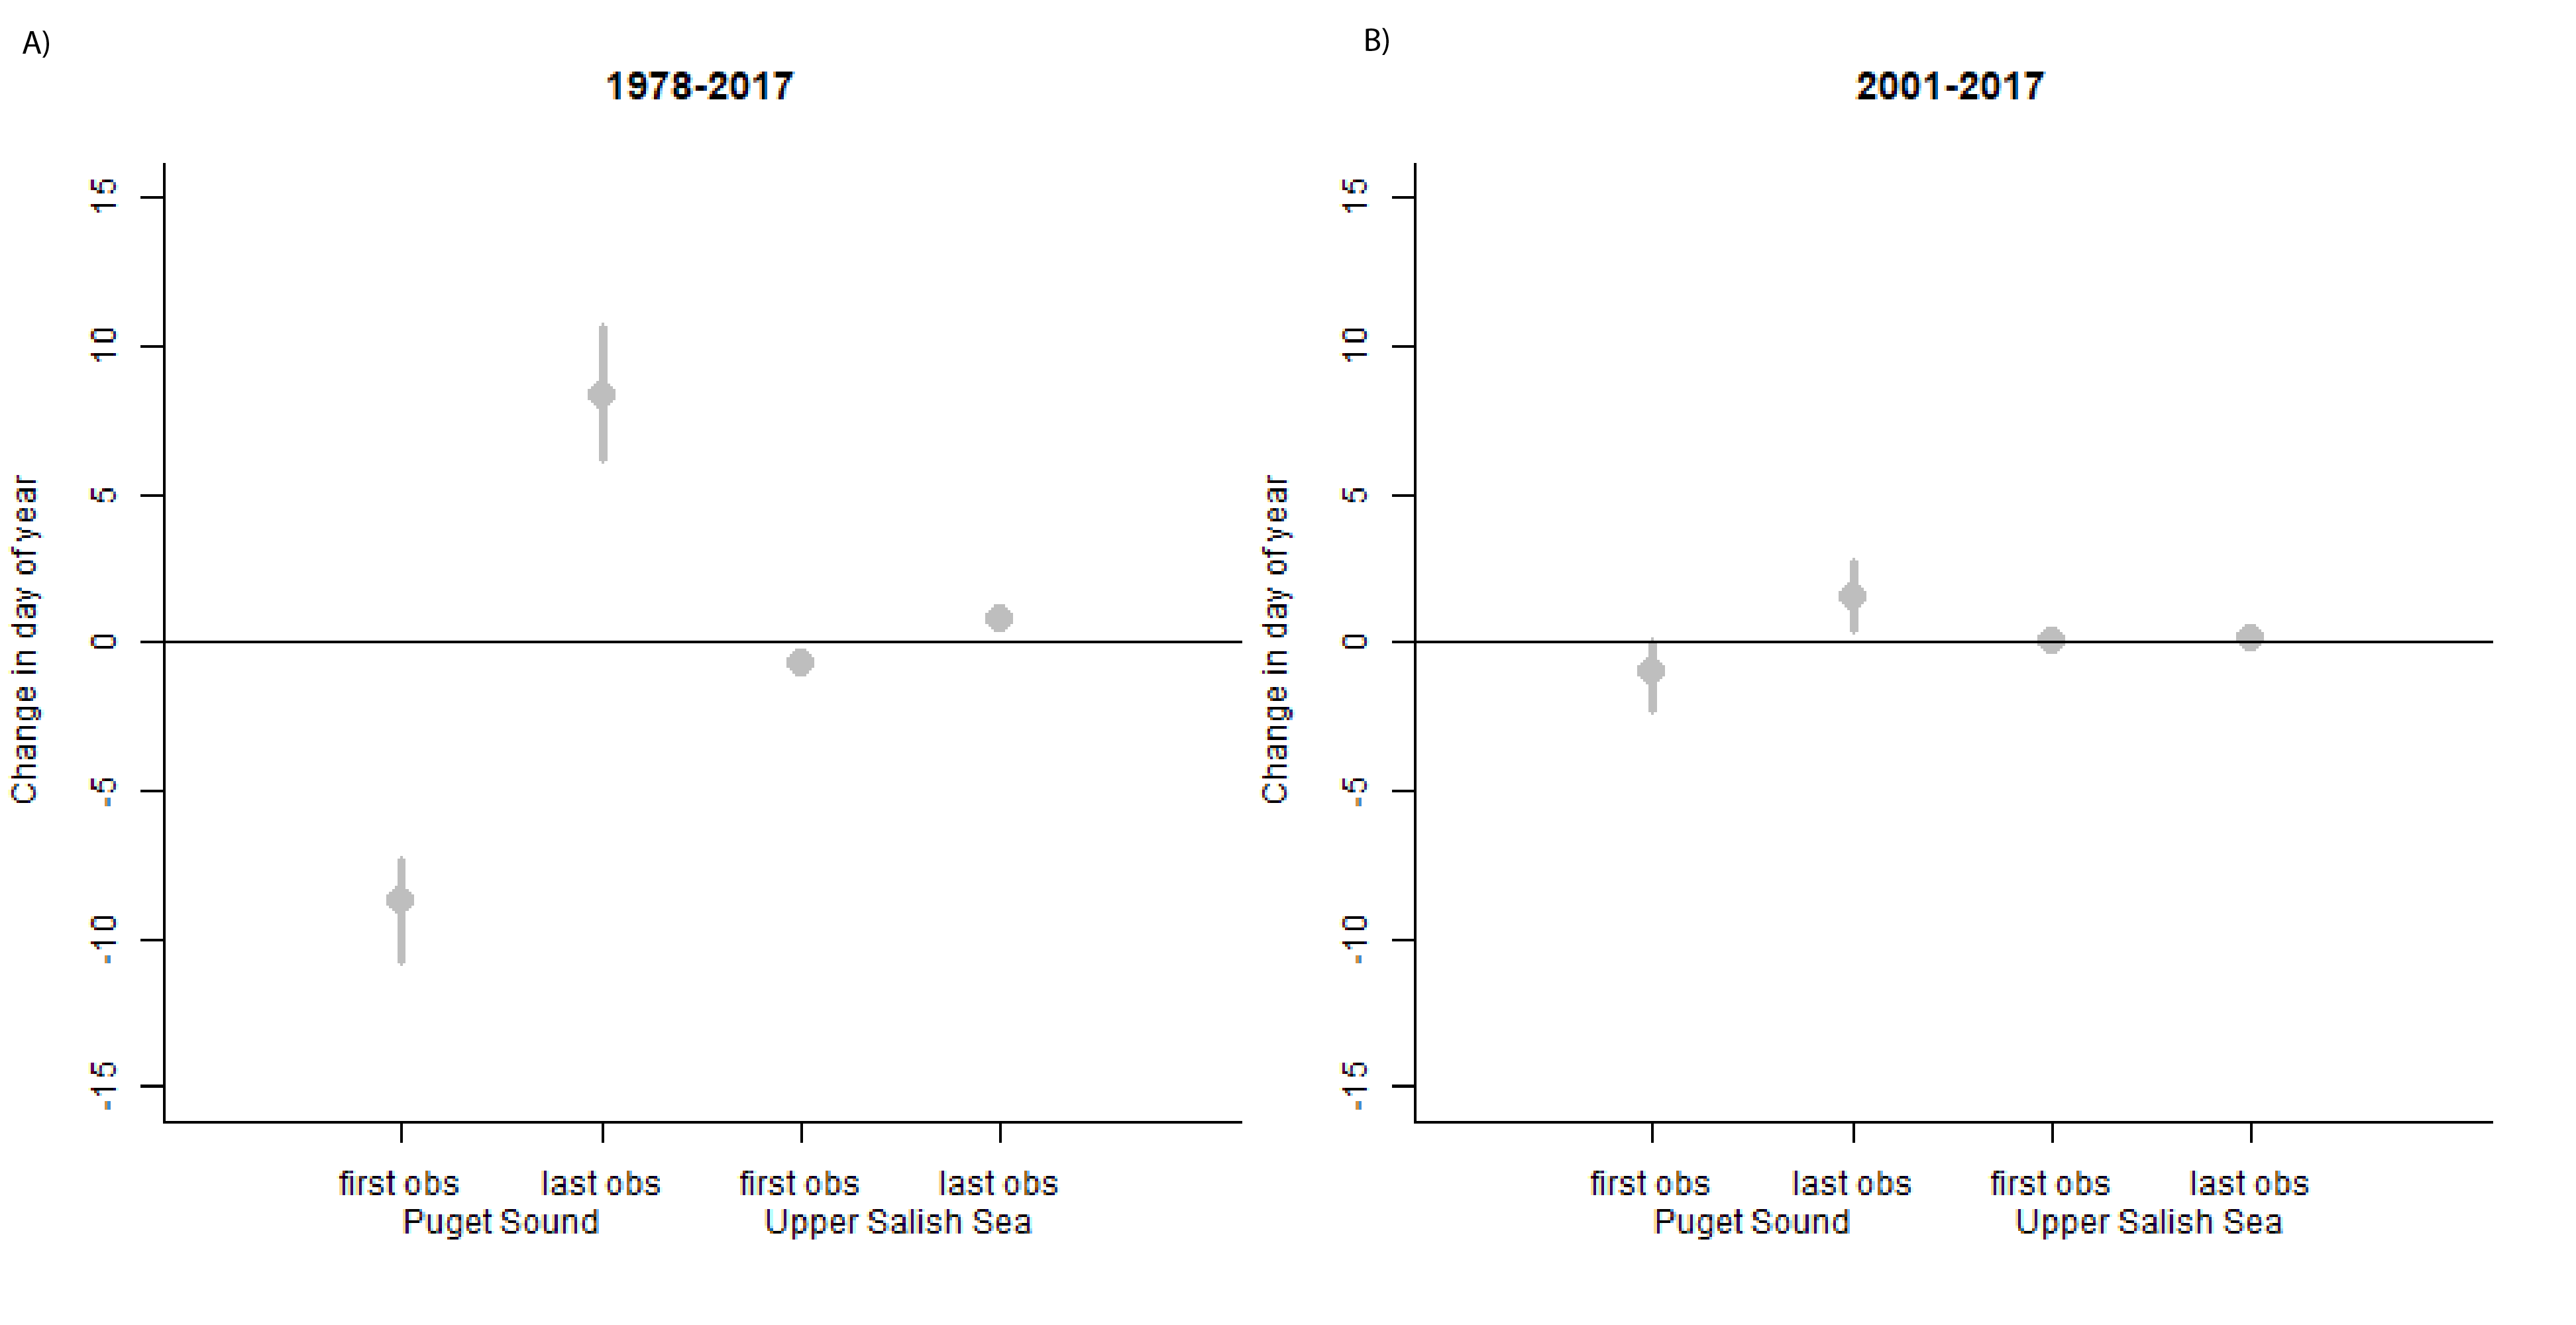
\includegraphics[width=0.8\textwidth]{../analyses/orcaphen/figures/simeffortonly2panels.png} 
\caption{\textbf{Expected change in phenology due to changes in effort alone, across Puget Sound and the Central Salish Sea regions}, from 1978-2017 (A) and from 2001-2017 (B).Error bars represent 75\% uncertainty intervals. }
\label{fig:simeffort}
\end{figure}

\pagebreak


%%%%%%%%%%%%%%%%%%%%%%%%%%%%%%%%%%%%%%
  \end{document}
%%%%%%%%%%%%%%%%%%%%%%%%%%%%%%%%%%%%%%
